\documentclass[]{article}
\usepackage{lmodern}
\usepackage{amssymb,amsmath}
\usepackage{ifxetex,ifluatex}
\usepackage{fixltx2e} % provides \textsubscript
\ifnum 0\ifxetex 1\fi\ifluatex 1\fi=0 % if pdftex
  \usepackage[T1]{fontenc}
  \usepackage[utf8]{inputenc}
\else % if luatex or xelatex
  \ifxetex
    \usepackage{mathspec}
  \else
    \usepackage{fontspec}
  \fi
  \defaultfontfeatures{Ligatures=TeX,Scale=MatchLowercase}
\fi
% use upquote if available, for straight quotes in verbatim environments
\IfFileExists{upquote.sty}{\usepackage{upquote}}{}
% use microtype if available
\IfFileExists{microtype.sty}{%
\usepackage{microtype}
\UseMicrotypeSet[protrusion]{basicmath} % disable protrusion for tt fonts
}{}
\usepackage[margin=1in]{geometry}
\usepackage{hyperref}
\hypersetup{unicode=true,
            pdftitle={Modeling the Contribution of Offshore Wind to the Grid Mix and Air Quality Implications: National Approach Results and Analysis},
            pdfauthor={Morgan Browning},
            pdfborder={0 0 0},
            breaklinks=true}
\urlstyle{same}  % don't use monospace font for urls
\usepackage{graphicx,grffile}
\makeatletter
\def\maxwidth{\ifdim\Gin@nat@width>\linewidth\linewidth\else\Gin@nat@width\fi}
\def\maxheight{\ifdim\Gin@nat@height>\textheight\textheight\else\Gin@nat@height\fi}
\makeatother
% Scale images if necessary, so that they will not overflow the page
% margins by default, and it is still possible to overwrite the defaults
% using explicit options in \includegraphics[width, height, ...]{}
\setkeys{Gin}{width=\maxwidth,height=\maxheight,keepaspectratio}
\IfFileExists{parskip.sty}{%
\usepackage{parskip}
}{% else
\setlength{\parindent}{0pt}
\setlength{\parskip}{6pt plus 2pt minus 1pt}
}
\setlength{\emergencystretch}{3em}  % prevent overfull lines
\providecommand{\tightlist}{%
  \setlength{\itemsep}{0pt}\setlength{\parskip}{0pt}}
\setcounter{secnumdepth}{5}
% Redefines (sub)paragraphs to behave more like sections
\ifx\paragraph\undefined\else
\let\oldparagraph\paragraph
\renewcommand{\paragraph}[1]{\oldparagraph{#1}\mbox{}}
\fi
\ifx\subparagraph\undefined\else
\let\oldsubparagraph\subparagraph
\renewcommand{\subparagraph}[1]{\oldsubparagraph{#1}\mbox{}}
\fi

%%% Use protect on footnotes to avoid problems with footnotes in titles
\let\rmarkdownfootnote\footnote%
\def\footnote{\protect\rmarkdownfootnote}

%%% Change title format to be more compact
\usepackage{titling}

% Create subtitle command for use in maketitle
\providecommand{\subtitle}[1]{
  \posttitle{
    \begin{center}\large#1\end{center}
    }
}

\setlength{\droptitle}{-2em}

  \title{Modeling the Contribution of Offshore Wind to the Grid Mix and Air
Quality Implications: National Approach Results and Analysis}
    \pretitle{\vspace{\droptitle}\centering\huge}
  \posttitle{\par}
    \author{Morgan Browning}
    \preauthor{\centering\large\emph}
  \postauthor{\par}
      \predate{\centering\large\emph}
  \postdate{\par}
    \date{25 October, 2019}

\usepackage{booktabs}
\usepackage{longtable}
\usepackage{array}
\usepackage{multirow}
\usepackage{wrapfig}
\usepackage{float}
\usepackage{colortbl}
\usepackage{pdflscape}
\usepackage{tabu}
\usepackage{threeparttable}
\usepackage{threeparttablex}
\usepackage[normalem]{ulem}
\usepackage{makecell}
\usepackage{xcolor}
\usepackage{caption}
\usepackage{graphicx}
\usepackage{siunitx}
\usepackage{hhline}
\usepackage{calc}
\usepackage{tabularx}

\begin{document}
\maketitle

{
\setcounter{tocdepth}{2}
\tableofcontents
}
\begin{center}\rule{0.5\linewidth}{\linethickness}\end{center}

\hypertarget{disclosure}{%
\section{Disclosure}\label{disclosure}}

This document functions as an all-inclusive working directory for
synthesis and graphical analysis of the results from the offshore wind
research of Morgan Browning, an ORISE Fellow at the U.S. Environmental
Protection Agency's Office of Research and Development. This document
and its contents are not finalized nor are intended for publication.

It is annotated primarily for ease of reproducability and a general
understanding of the results.

\hypertarget{setup}{%
\section{Setup}\label{setup}}

Three scripts are loaded into this markdown document to allow for
analysis of the data. The setup script loads the library, creates
generalized functions, and creates global variables for color scales and
factors. The data script loads an excel spreadsheet with all of the
results data and performs the majority of data munging. The results
script creates charts, graphs, and tables. This report functions as the
annotated synthesis of the data and results.

Graphs are provided with many variations to meet criteria of different
publication and presentation platforms. Formats may be chosen using the
\texttt{colorcalls} toggles

\hypertarget{scenarios}{%
\section{Scenarios}\label{scenarios}}

The nested parametric sensitivity analysis was built on combinations of
two sets of scenarios:

\begin{enumerate}
\def\labelenumi{\arabic{enumi}.}
\tightlist
\item
  Electric sector CO\textsubscript{2} emissions caps, as a linear
  decrease to a given \% decrease from 2010 emissions by 2050\\
\end{enumerate}

\begin{itemize}
\tightlist
\item
  Business and usual emissions represent approximately a 20\% reduction
  in CO\textsubscript{2} emissions
\end{itemize}

\begin{enumerate}
\def\labelenumi{\arabic{enumi}.}
\setcounter{enumi}{1}
\tightlist
\item
  Cost reductions of offshore wind, as a linear decrease to a given \%
  decrease from 2010 costs by 2035, then level costs to 2050\\
\end{enumerate}

\begin{itemize}
\tightlist
\item
  A 20\% cost reduction is used as the base case, assuming very
  conservative technological advancement and little benefit of economies
  of scale
\item
  Cost curves are set to resolve by 2035 as estimated based on NREL LCOE
  cost projections for offshore wind
\end{itemize}

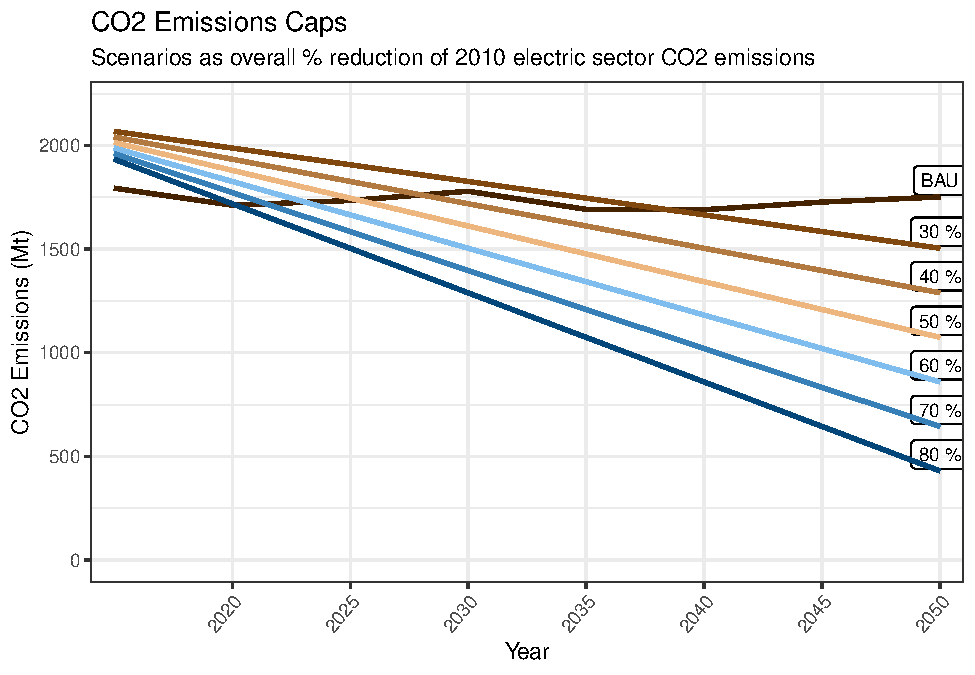
\includegraphics[width=0.5\linewidth]{osw_Report_files/figure-latex/unnamed-chunk-4-1}
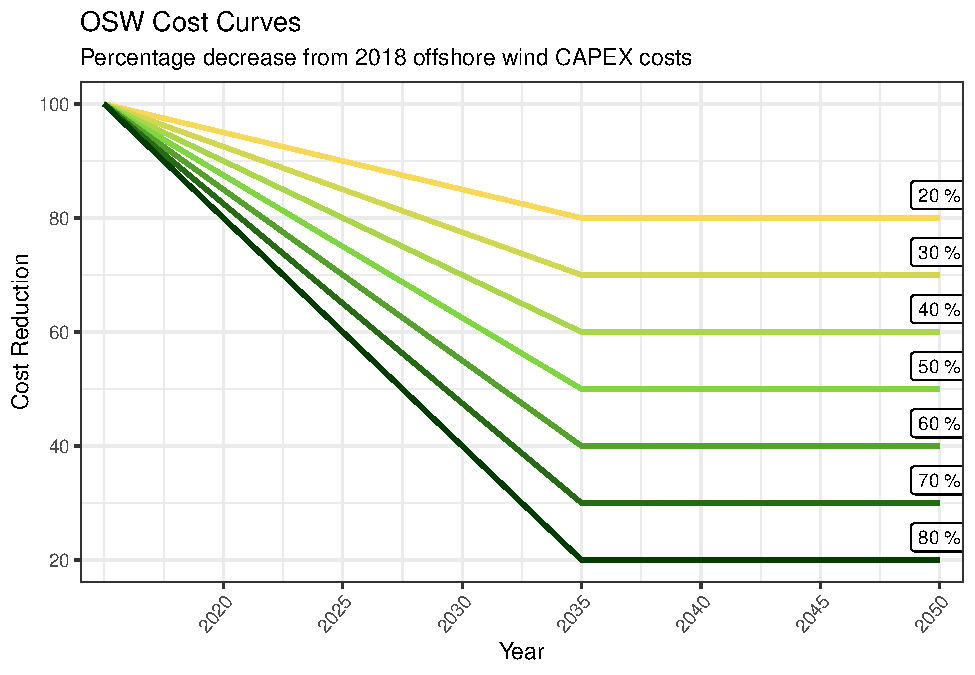
\includegraphics[width=0.5\linewidth]{osw_Report_files/figure-latex/unnamed-chunk-4-2}

\hypertarget{lcoe}{%
\section{LCOE}\label{lcoe}}

EIA's AEO 2019 provides the following values for the estimated levelized
cost of electricity (capacity-weighted average) for new generation
resources entering service in 2023 (2018 \$/MWh). Offshore wind has the
highest total LCOE by a large margin. The second most expensive
technology is biomass. The AEO LCOE was used in the calculation of
offshore wind costs for the above cost curves, but LCOE is not directly
used in the model.

\begin{table}[!h]

\caption{\label{tab:unnamed-chunk-3}Estimated LCOE capacity-weighted average for new generation 
        resources entering service in 2023 (2018 \$/MWh)}
\centering
\resizebox{\linewidth}{!}{
\begin{tabular}{>{\raggedright\arraybackslash}p{2.95 cm}>{\raggedleft\arraybackslash}p{1.2 cm}>{\raggedleft\arraybackslash}p{1.2 cm}>{\raggedleft\arraybackslash}p{1.2 cm}>{\raggedleft\arraybackslash}p{1.2 cm}>{\raggedleft\arraybackslash}p{1.2 cm}>{\raggedleft\arraybackslash}p{1.2 cm}>{\raggedright\arraybackslash}p{1.2 cm}>{\raggedleft\arraybackslash}p{1.5 cm}}
\toprule
Plant Type & Capacity Factor (\%) & Levelized capital cost & Levelized fixed O\&M & Levelized variable O\&M & Levelized transmission cost & Total system LCOE & Levelized tax credit & Total LCOE including tax credit\\
\midrule
\rowcolor{gray!6}  \addlinespace[0.3em]
\multicolumn{9}{l}{\textbf{Dispatchable technologies}}\\
\hspace{1em}Conventional CC & 87 & 8.1 & 1.5 & 32.3 & 0.9 & 42.8 & NA & 42.8\\
\hspace{1em}Advanced CC & 87 & 7.1 & 1.4 & 30.7 & 1.0 & 40.2 & NA & 40.2\\
\rowcolor{gray!6}  \hspace{1em}Advanced CT & 30 & 17.2 & 2.7 & 54.6 & 3.0 & 77.5 & NA & 77.5\\
\hspace{1em}Geothermal & 90 & 24.6 & 13.3 & 0.0 & 1.4 & 39.4 & -2.5 & 36.9\\
\rowcolor{gray!6}  \hspace{1em}Biomass & 83 & 37.3 & 15.7 & 37.5 & 1.5 & 92.1 & NA & 92.1\\
\addlinespace[0.3em]
\multicolumn{9}{l}{\textbf{Non-dispatchable technologies}}\\
\hspace{1em}Wind, onshore & 44 & 27.8 & 12.6 & 0.0 & 2.4 & 42.8 & -6.1 & 36.6\\
\rowcolor{gray!6}  \hspace{1em}Wind, offshore & 45 & 95.5 & 20.4 & 0.0 & 2.1 & 117.9 & -11.5 & 106.5\\
\hspace{1em}Solar PV & 29 & 37.1 & 8.8 & 0.0 & 2.9 & 48.8 & -11.5 & 37.6\\
\rowcolor{gray!6}  \hspace{1em}Hydroelectric & 75 & 29.9 & 6.2 & 1.4 & 1.6 & 39.1 & NA & 39.1\\
\bottomrule
\multicolumn{9}{l}{\textit{Note: }}\\
\multicolumn{9}{l}{U.S. EIA Annual Energy Outlook 2019}\\
\end{tabular}}
\end{table}

\hypertarget{offshore-wind}{%
\section{Offshore Wind}\label{offshore-wind}}

As offshore wind is the primary technology being assessed in this
research, we have explored many facets of offshore wind buildout. These
facets are explored below, both at a regional and national cumulative
level.

\hypertarget{capacity-buildout}{%
\subsection{Capacity Buildout}\label{capacity-buildout}}

Cumulative and new addition offshore wind capacity across all nine
census regions, by cost and emissions reduction scenario.

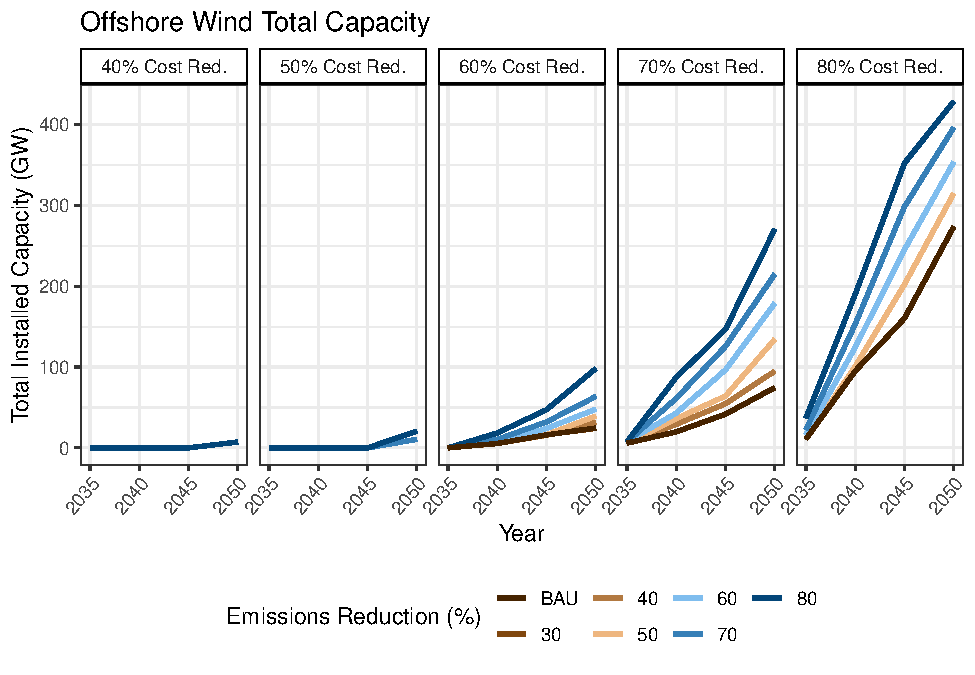
\includegraphics[width=0.5\linewidth]{osw_Report_files/figure-latex/unnamed-chunk-7-1}
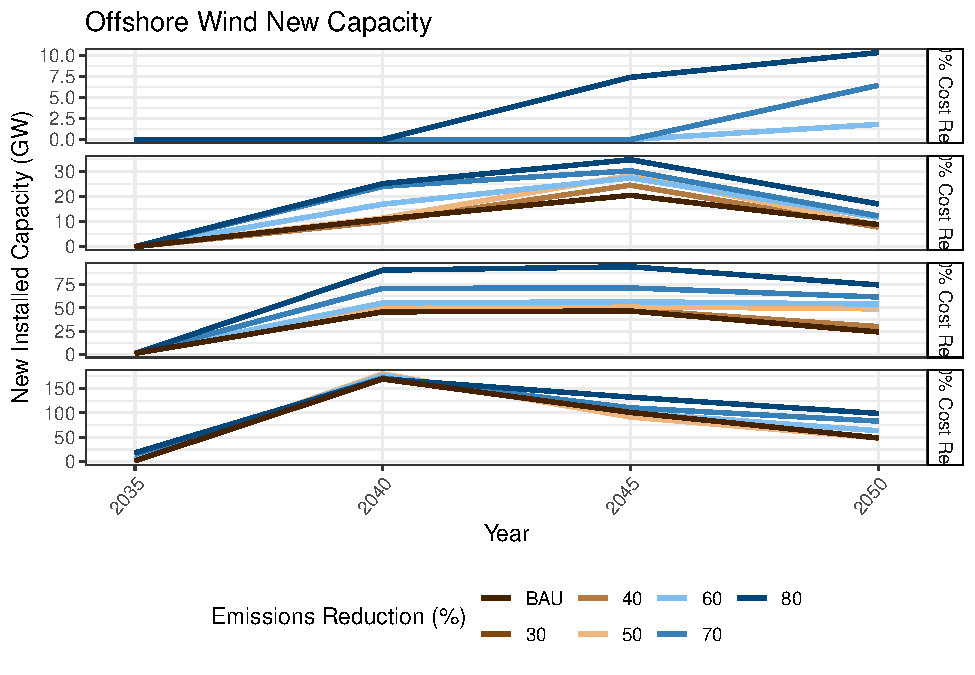
\includegraphics[width=0.5\linewidth]{osw_Report_files/figure-latex/unnamed-chunk-7-2}

\hypertarget{total-capacity}{%
\subsection{Total Capacity}\label{total-capacity}}

Total offshore wind capacity across all nine census regions in 2050, by
cost and emissions reduction scenario.

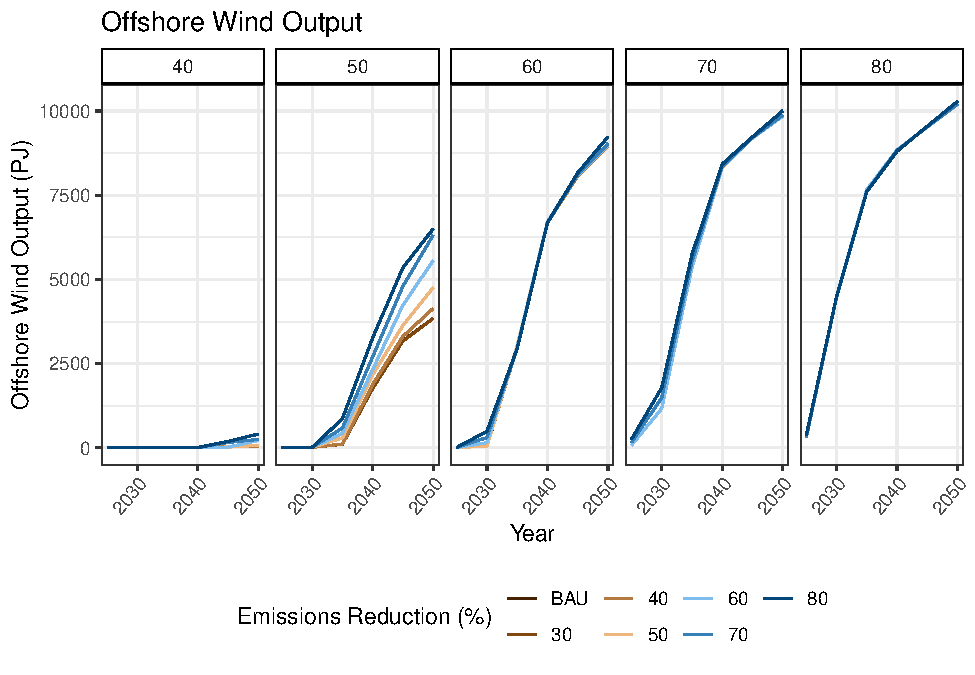
\includegraphics{osw_Report_files/figure-latex/unnamed-chunk-10-1.pdf}

\begin{table}[!h]

\caption{\label{tab:unnamed-chunk-3}Offshore Wind Total Installed Capacity (GW): 2050}
\centering
\begin{tabular}{lrrrr}
\toprule
\multicolumn{1}{c}{\makecell[c]{CO2 Emissions\\Reduction (\%)}} & \multicolumn{4}{c}{Cost Reduction (\%)} \\
\cmidrule(l{3pt}r{3pt}){1-1} \cmidrule(l{3pt}r{3pt}){2-5}
 & 50 & 60 & 70 & 80\\
\midrule
\rowcolor{gray!6}  BAU & NA & 40.1 & 117.8 & 320.4\\
30 & NA & 40.1 & 117.8 & 320.4\\
\rowcolor{gray!6}  40 & NA & 42.2 & 125.6 & 320.4\\
50 & NA & 48.3 & 150.5 & 321.4\\
\rowcolor{gray!6}  60 & 1.8 & 55.8 & 166.7 & 345.5\\
70 & 6.4 & 66.3 & 204.4 & 380.1\\
\rowcolor{gray!6}  80 & 17.7 & 76.6 & 259.6 & 418.6\\
\bottomrule
\end{tabular}
\end{table}

\hypertarget{output}{%
\subsection{Output}\label{output}}

Total offshore wind electricity output across all nine census regions,
by cost and emissions reduction scenario. Results show almost identical
trajectories for total capacity and output due to the non-dispatchable
quality of offshore wind. All generated electricity is utilized in the
modeled scenarios.

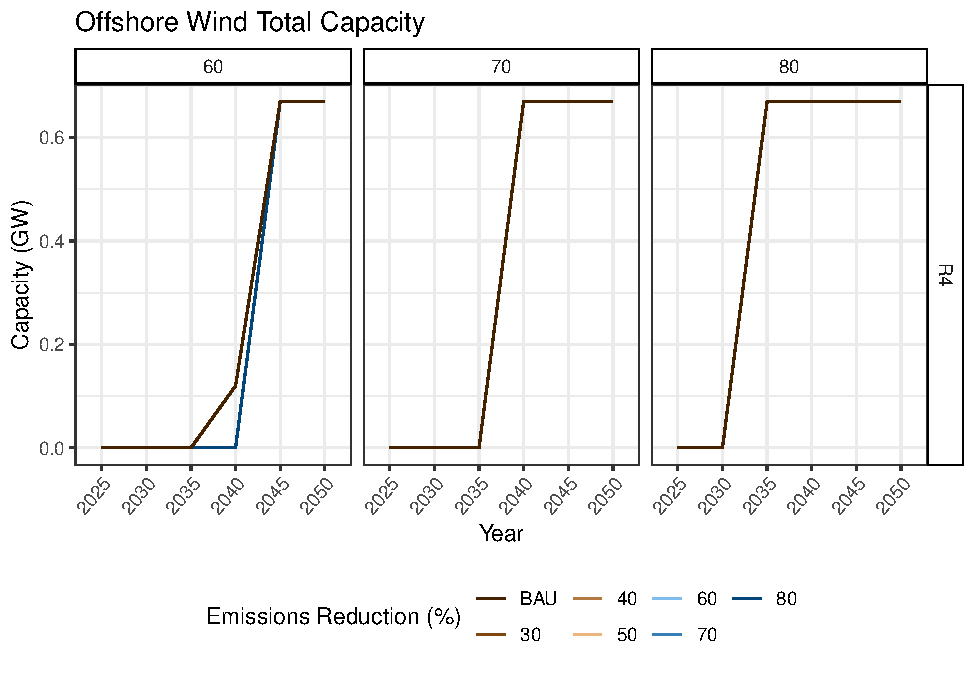
\includegraphics{osw_Report_files/figure-latex/unnamed-chunk-12-1.pdf}

\begin{table}[!h]

\caption{\label{tab:unnamed-chunk-3}Offshore Wind Total Output (PJ): 2050}
\centering
\begin{tabular}{lrrrr}
\toprule
\multicolumn{1}{c}{\makecell[c]{CO2 Emissions\\Reduction (\%)}} & \multicolumn{4}{c}{Cost Reduction (\%)} \\
\cmidrule(l{3pt}r{3pt}){1-1} \cmidrule(l{3pt}r{3pt}){2-5}
 & 50 & 60 & 70 & 80\\
\midrule
\rowcolor{gray!6}  BAU & NA & 661.5 & 1881.1 & 4902.4\\
30 & NA & 661.5 & 1881.1 & 4902.4\\
\rowcolor{gray!6}  40 & NA & 696.8 & 2001.7 & 4902.4\\
50 & NA & 797.6 & 2387.9 & 4917.0\\
\rowcolor{gray!6}  60 & 29.4 & 915.7 & 2648.6 & 5263.3\\
70 & 105.9 & 1079.9 & 3217.6 & 5761.1\\
\rowcolor{gray!6}  80 & 292.3 & 1242.4 & 4003.5 & 6285.8\\
\bottomrule
\end{tabular}
\end{table}

\hypertarget{regions}{%
\subsection{Regions}\label{regions}}

Cumulative and new addition offshore wind capacity by region. Regions
are listed from least to highest electricity output.

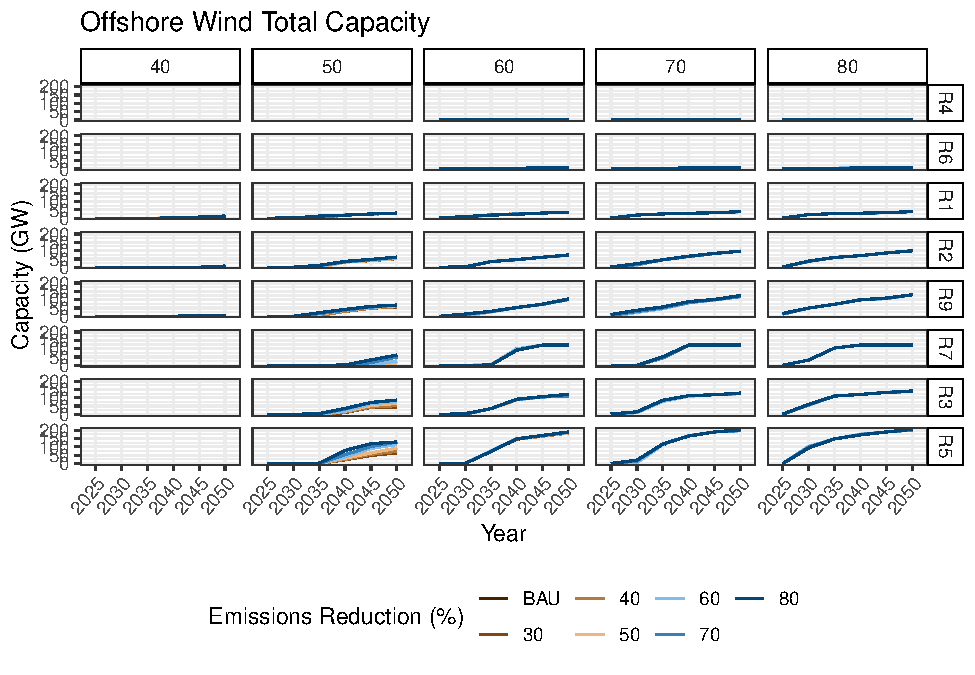
\includegraphics[width=0.5\linewidth]{osw_Report_files/figure-latex/unnamed-chunk-14-1}
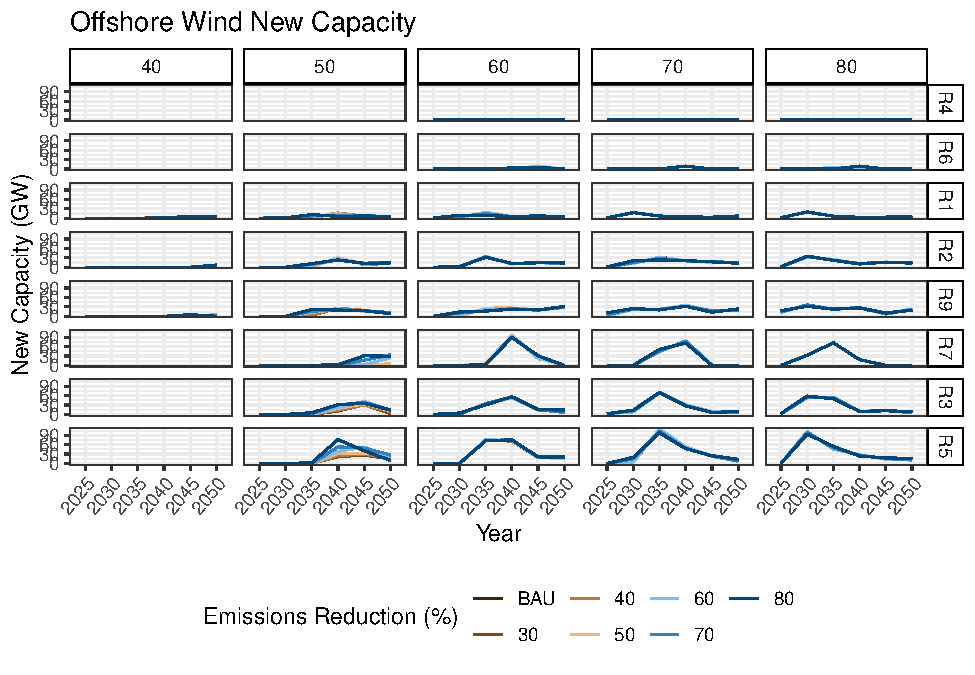
\includegraphics[width=0.5\linewidth]{osw_Report_files/figure-latex/unnamed-chunk-14-2}
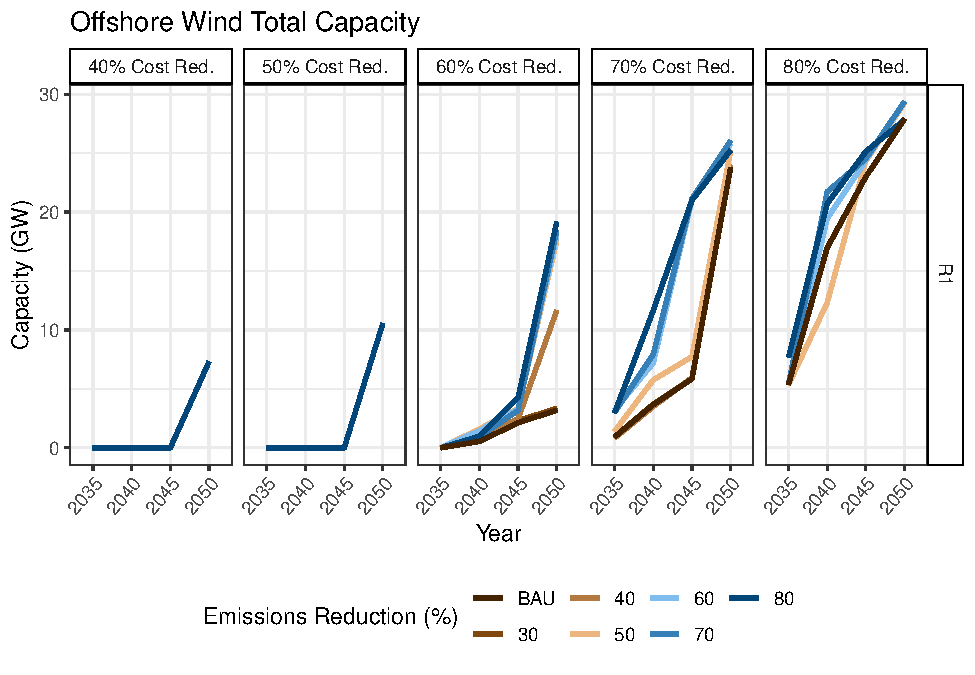
\includegraphics[width=0.5\linewidth]{osw_Report_files/figure-latex/unnamed-chunk-14-3}
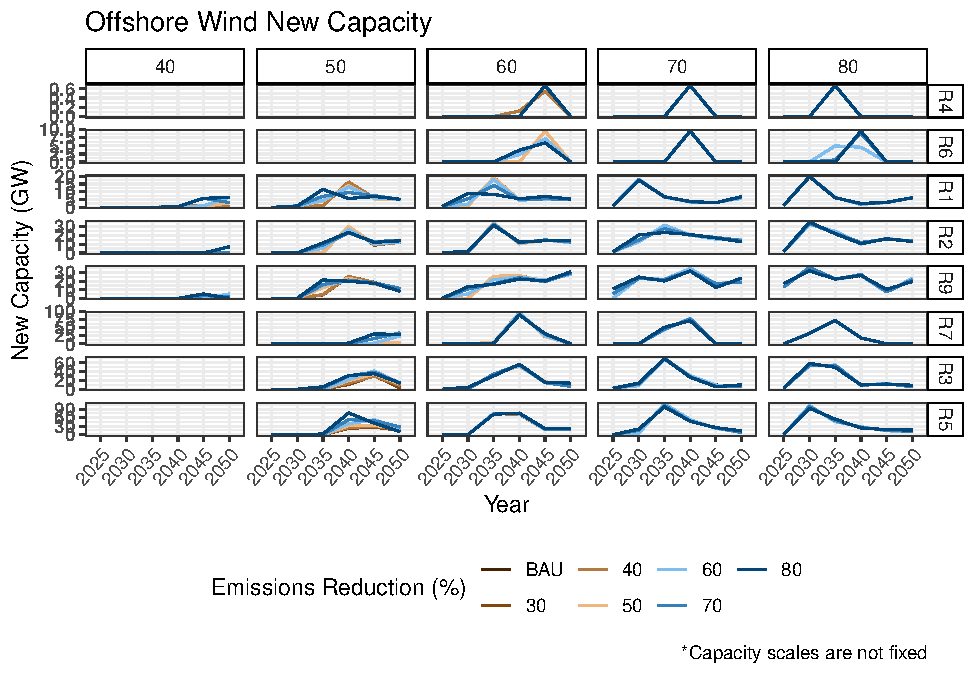
\includegraphics[width=0.5\linewidth]{osw_Report_files/figure-latex/unnamed-chunk-14-4}
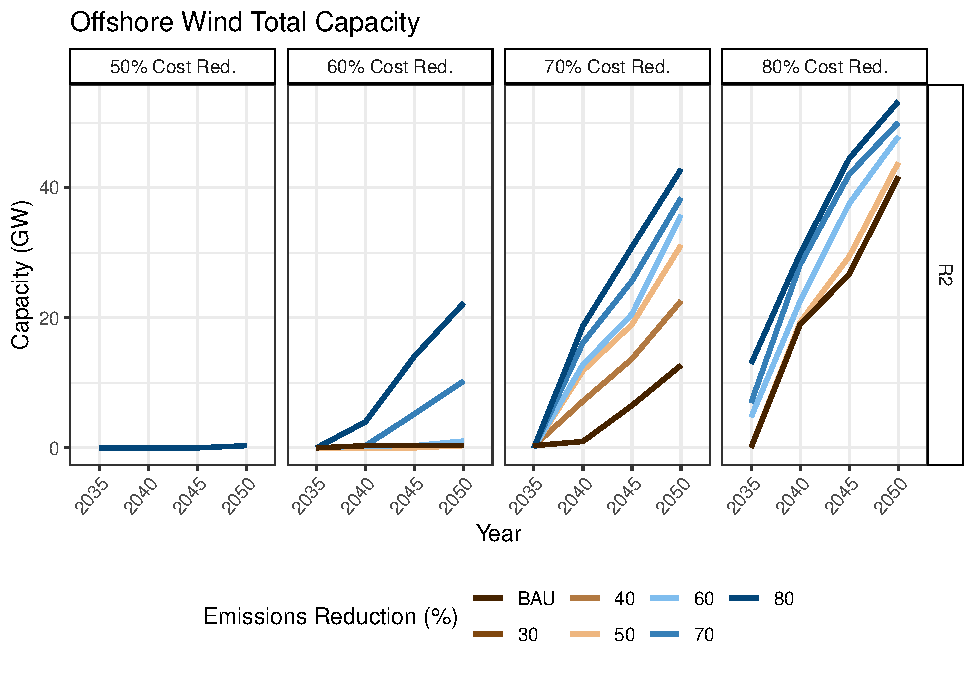
\includegraphics[width=0.5\linewidth]{osw_Report_files/figure-latex/unnamed-chunk-14-5}
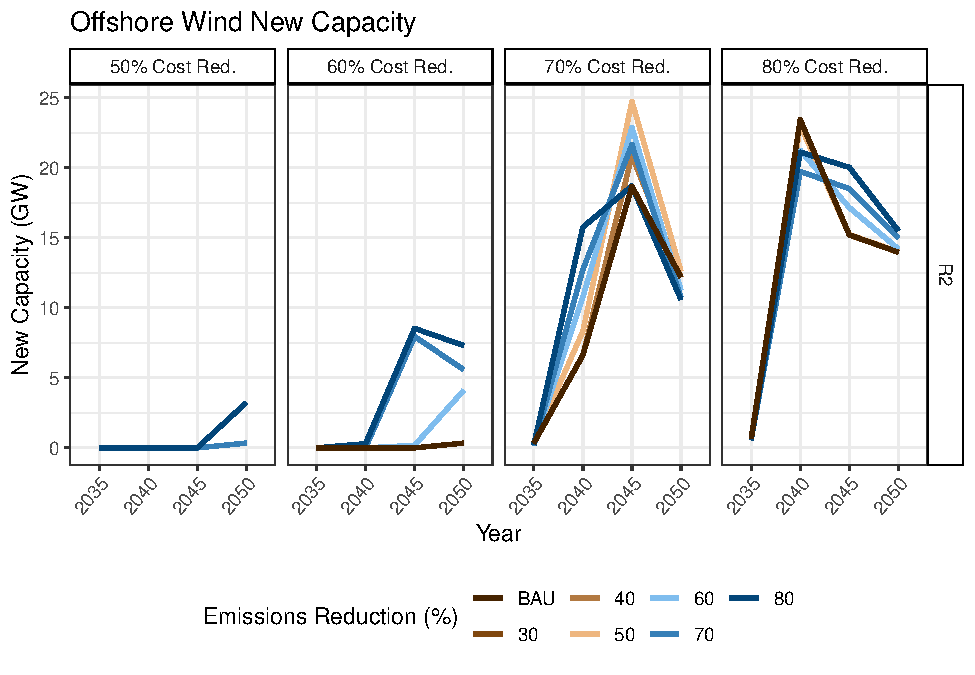
\includegraphics[width=0.5\linewidth]{osw_Report_files/figure-latex/unnamed-chunk-14-6}
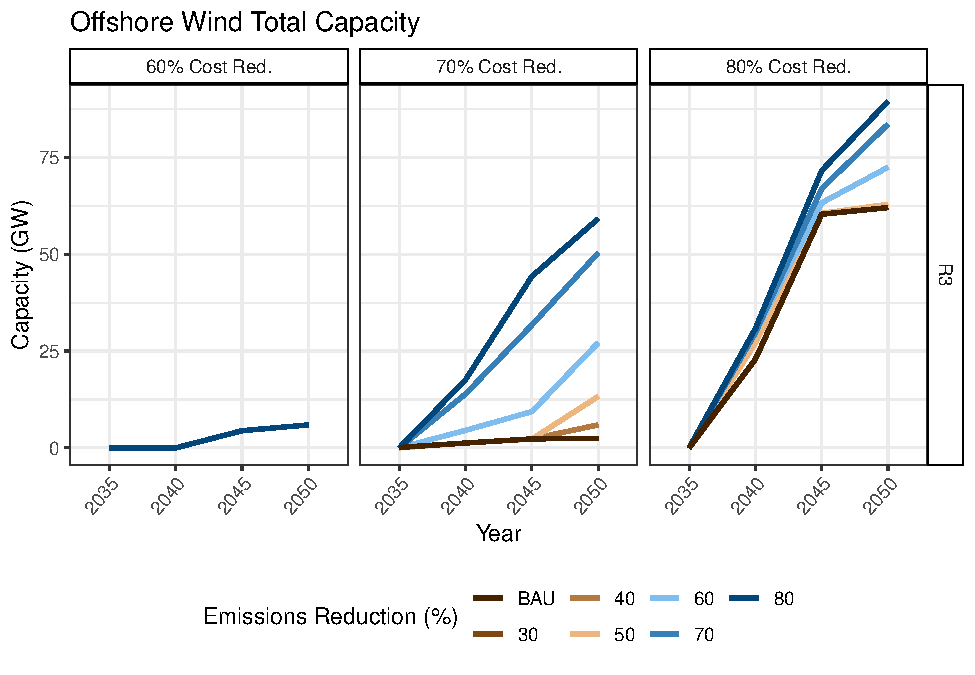
\includegraphics[width=0.5\linewidth]{osw_Report_files/figure-latex/unnamed-chunk-14-7}
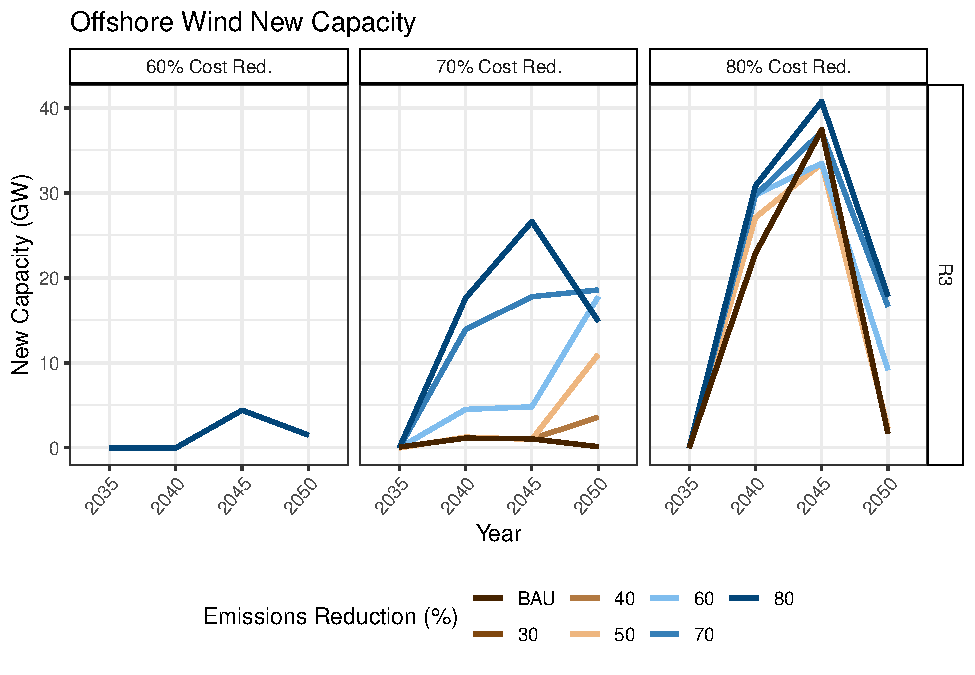
\includegraphics[width=0.5\linewidth]{osw_Report_files/figure-latex/unnamed-chunk-14-8}
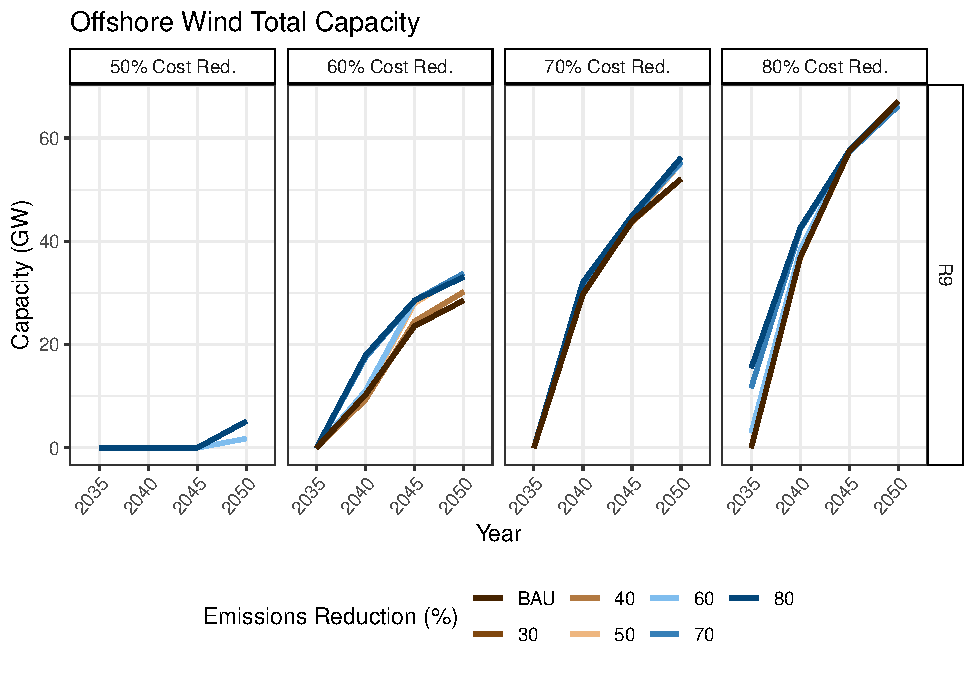
\includegraphics[width=0.5\linewidth]{osw_Report_files/figure-latex/unnamed-chunk-14-9}
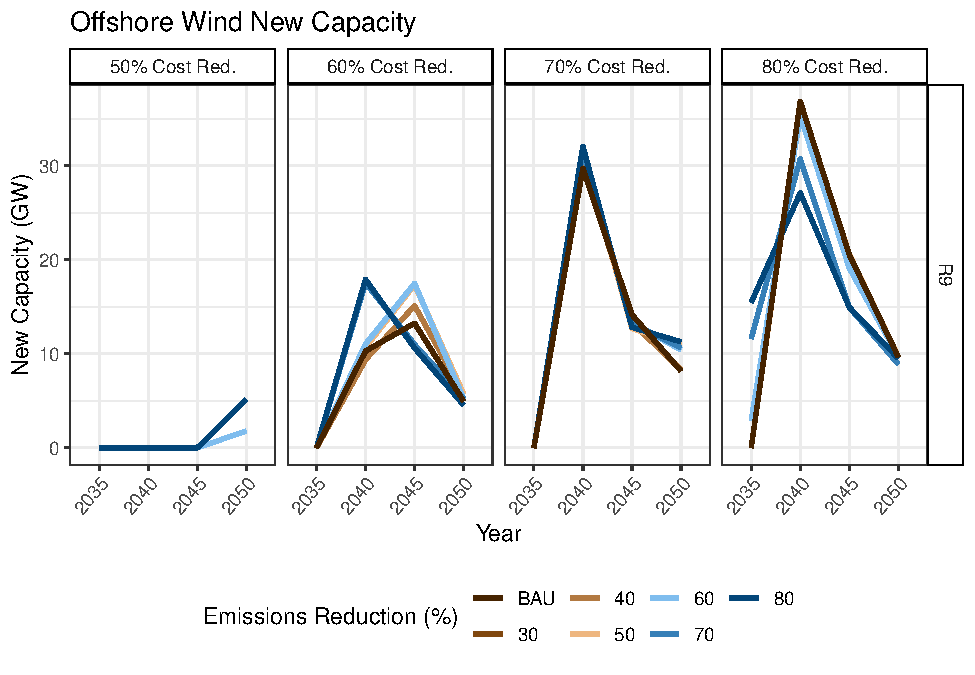
\includegraphics[width=0.5\linewidth]{osw_Report_files/figure-latex/unnamed-chunk-14-10}
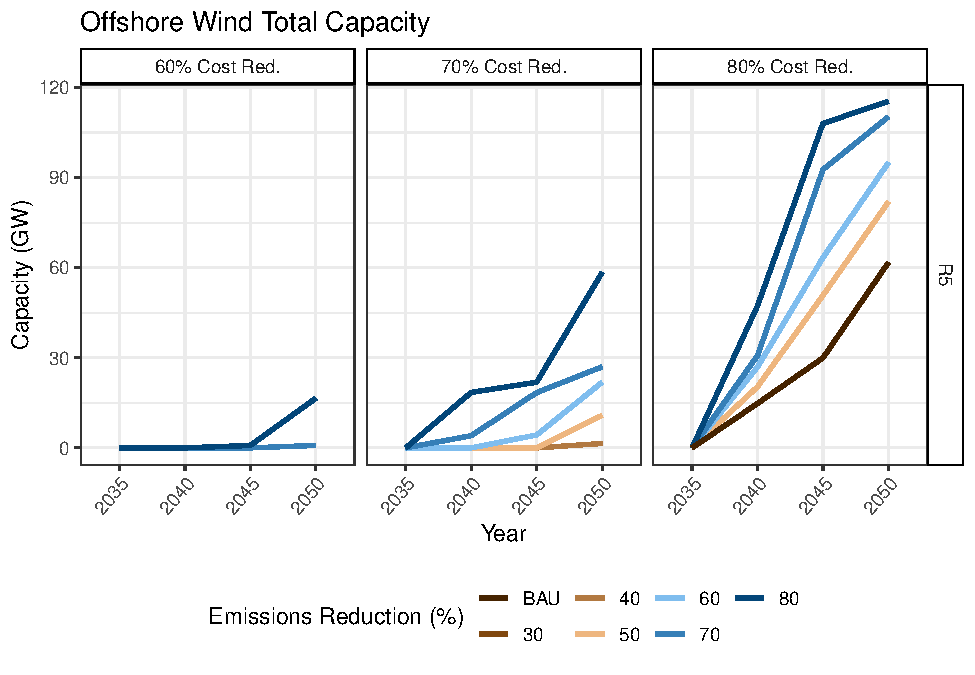
\includegraphics[width=0.5\linewidth]{osw_Report_files/figure-latex/unnamed-chunk-14-11}
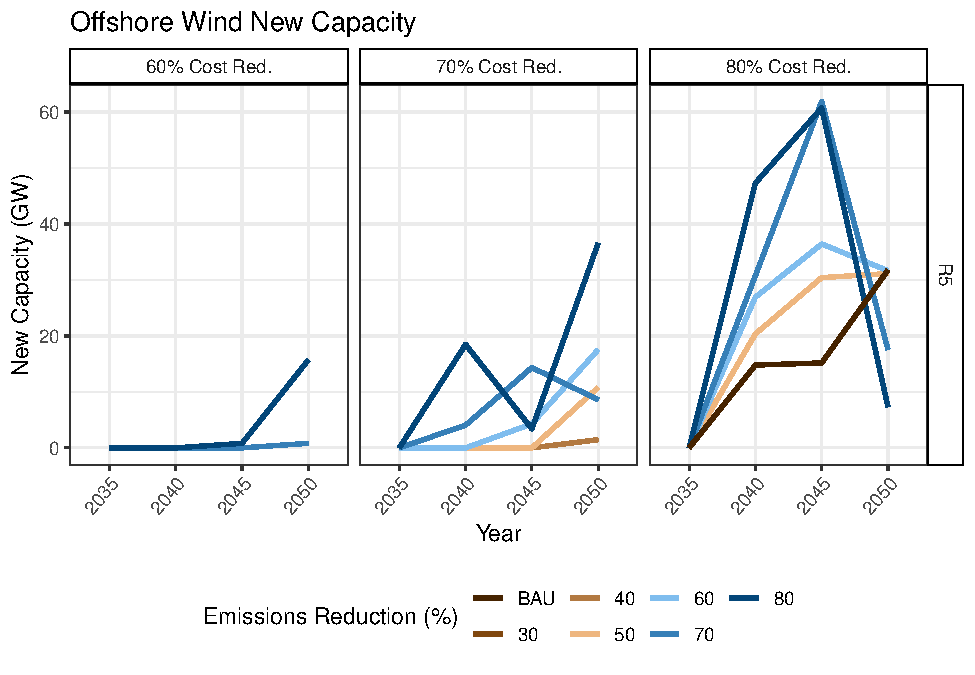
\includegraphics[width=0.5\linewidth]{osw_Report_files/figure-latex/unnamed-chunk-14-12}

Cumulative and new addition offshore wind capacity by region, emissions
reduction, and cost reduction.

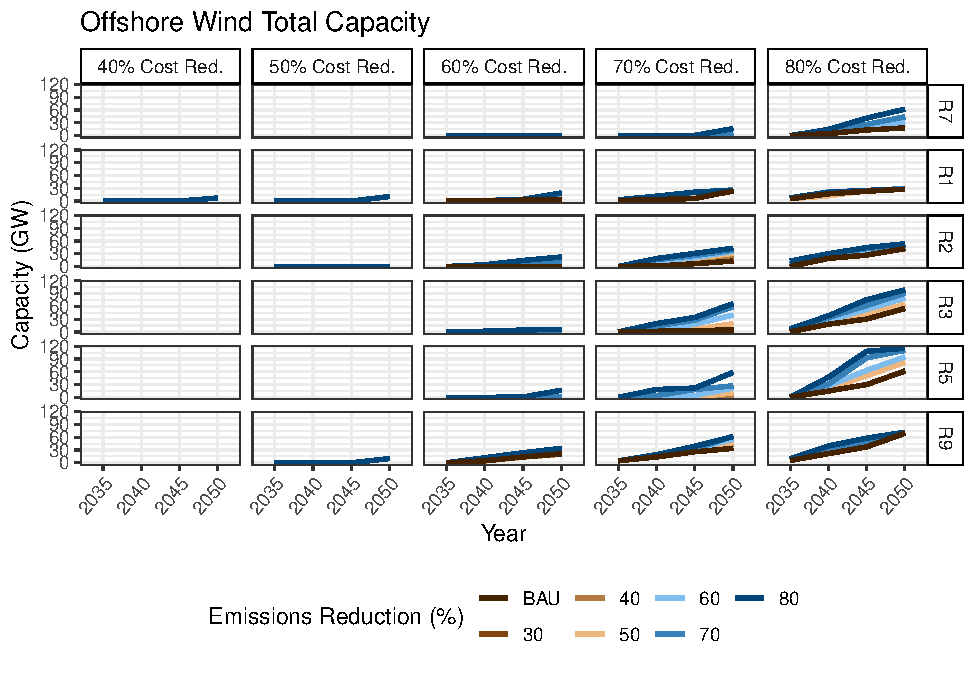
\includegraphics[width=0.5\linewidth]{osw_Report_files/figure-latex/unnamed-chunk-16-1}
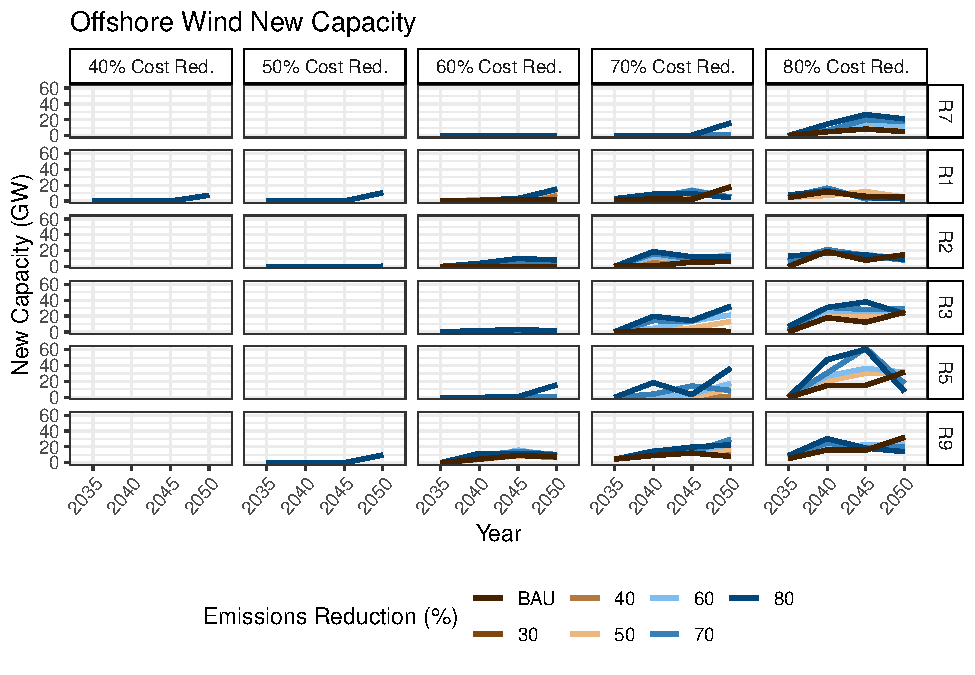
\includegraphics[width=0.5\linewidth]{osw_Report_files/figure-latex/unnamed-chunk-16-2}
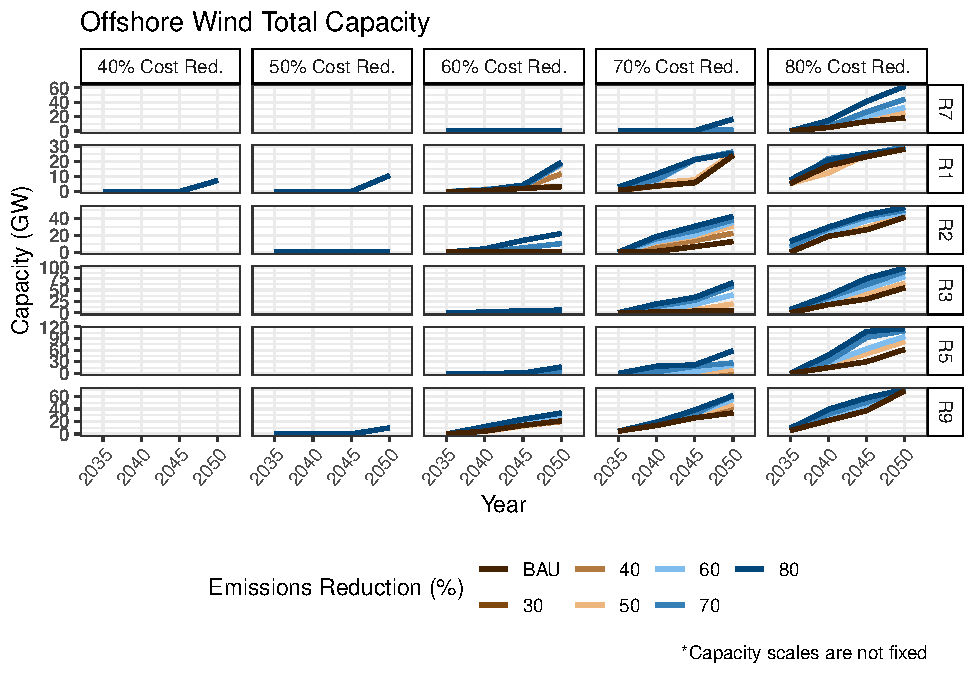
\includegraphics[width=0.5\linewidth]{osw_Report_files/figure-latex/unnamed-chunk-16-3}
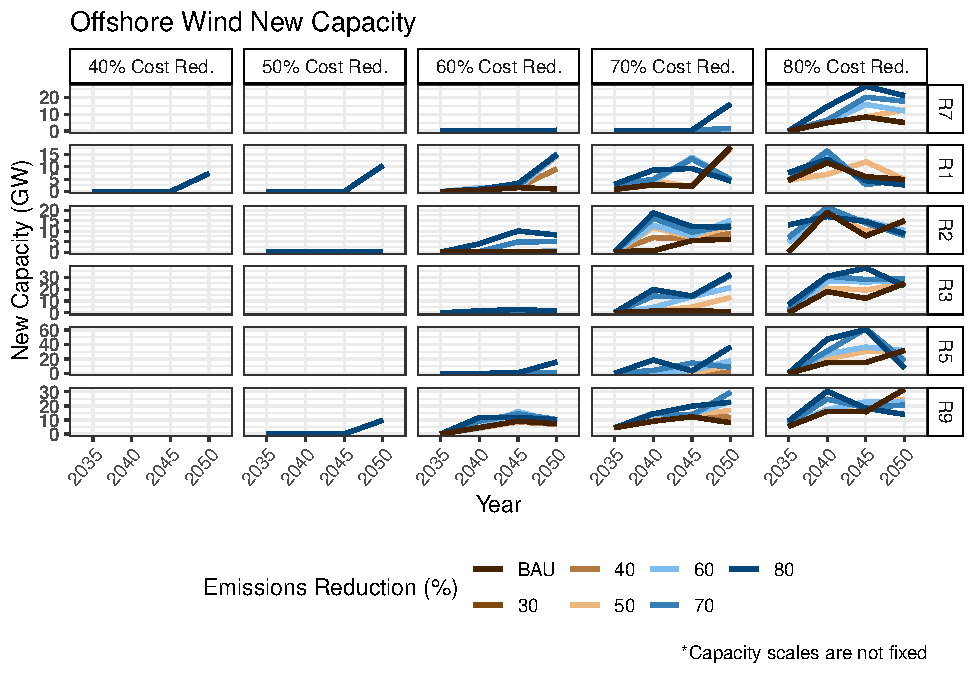
\includegraphics[width=0.5\linewidth]{osw_Report_files/figure-latex/unnamed-chunk-16-4}

\begin{table}[!h]

\caption{\label{tab:unnamed-chunk-3}Average Installed Capacity (GW)}
\centering
\begin{tabular}{lr}
\toprule
Region & 2050 Total\\
\midrule
\rowcolor{gray!6}  R7 & 20.73100\\
R1 & 21.50304\\
\rowcolor{gray!6}  R2 & 31.02391\\
R3 & 44.07267\\
\rowcolor{gray!6}  R9 & 45.02875\\
R5 & 50.47438\\
\bottomrule
\multicolumn{2}{l}{\textit{Note: }}\\
\multicolumn{2}{l}{Average is across all scenarios}\\
\end{tabular}
\end{table}

\begin{table}[!h]

\caption{\label{tab:unnamed-chunk-3}Average Electricity Output (PJ)}
\centering
\begin{tabular}{lr}
\toprule
Region & 2050 Total\\
\midrule
\rowcolor{gray!6}  R1 & 103.8590\\
R7 & 120.4272\\
\rowcolor{gray!6}  R2 & 157.8955\\
R3 & 216.6808\\
\rowcolor{gray!6}  R9 & 251.5586\\
R5 & 318.5086\\
\bottomrule
\multicolumn{2}{l}{\textit{Note: }}\\
\multicolumn{2}{l}{Average is across all scenarios}\\
\end{tabular}
\end{table}

Map of average total capacity

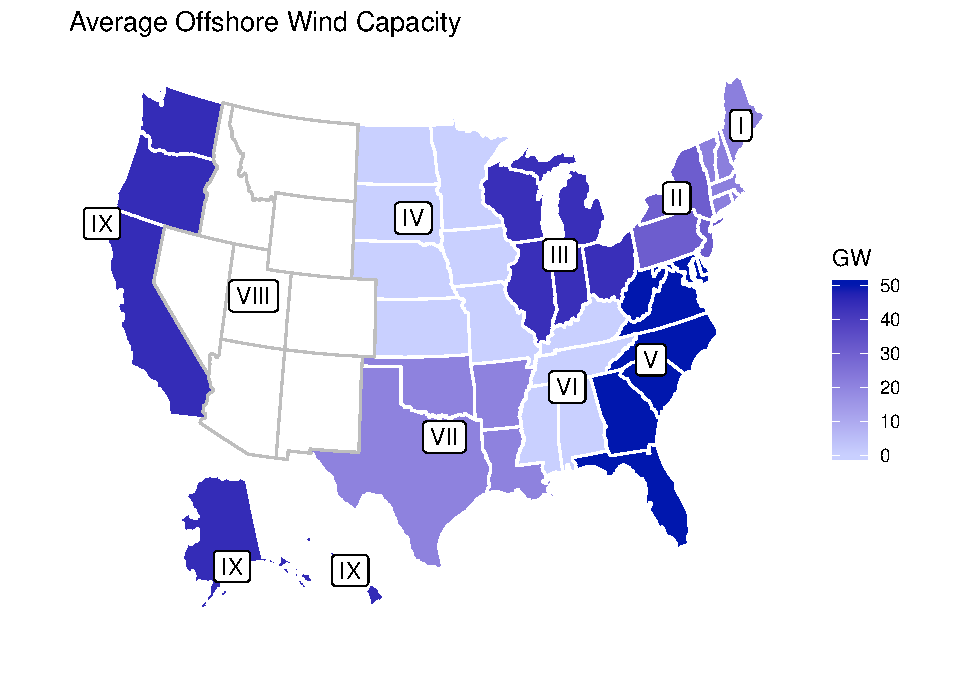
\includegraphics{osw_Report_files/figure-latex/unnamed-chunk-19-1.pdf}

\hypertarget{grid-mix}{%
\section{Grid Mix}\label{grid-mix}}

\hypertarget{baseline-production}{%
\subsection{Baseline Production}\label{baseline-production}}

Grid mix without any offshore wind cost reduction or emissions cap.

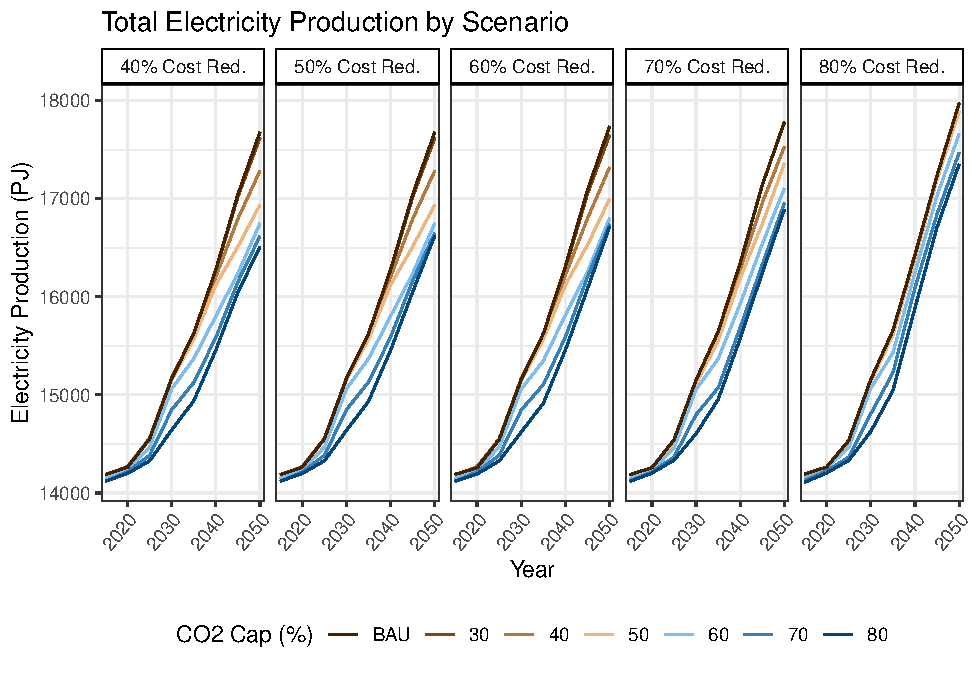
\includegraphics[width=0.5\linewidth]{osw_Report_files/figure-latex/unnamed-chunk-20-1}
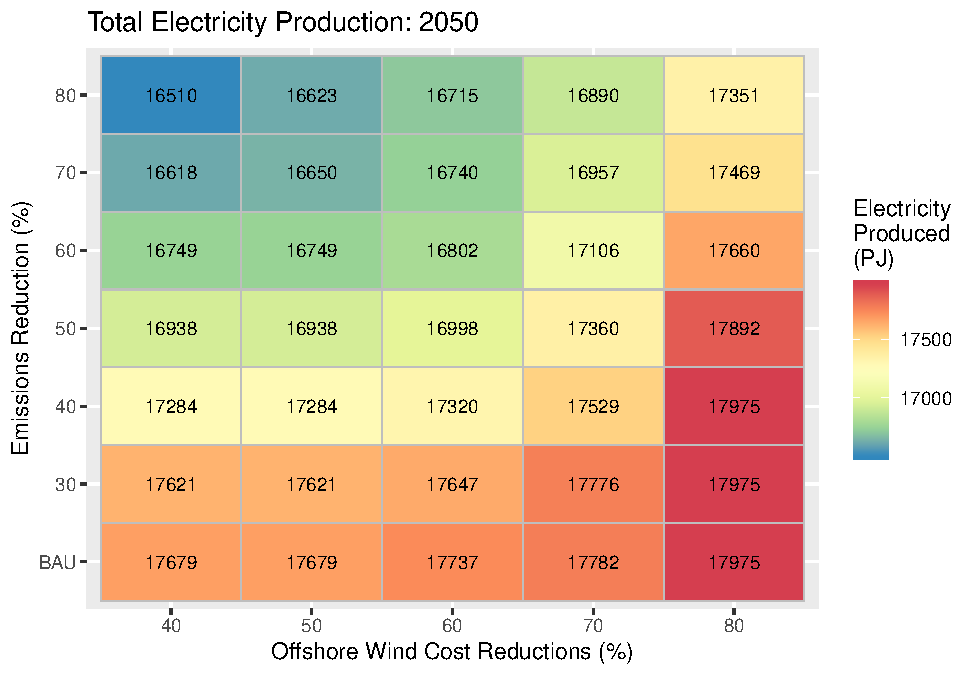
\includegraphics[width=0.5\linewidth]{osw_Report_files/figure-latex/unnamed-chunk-20-2}

Regional baseline production

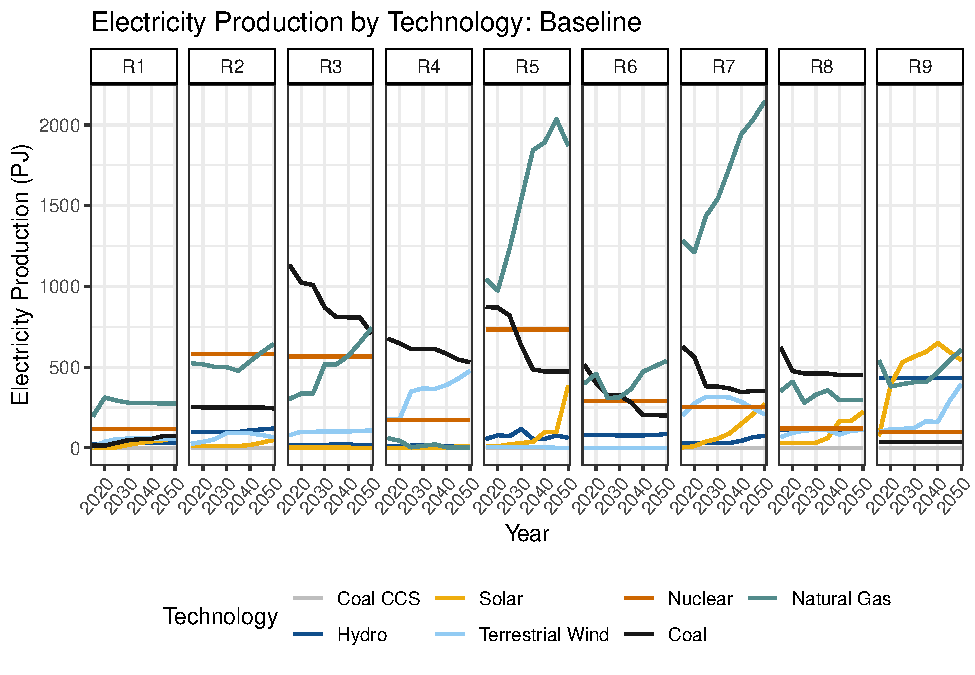
\includegraphics[width=0.5\linewidth]{osw_Report_files/figure-latex/unnamed-chunk-22-1}
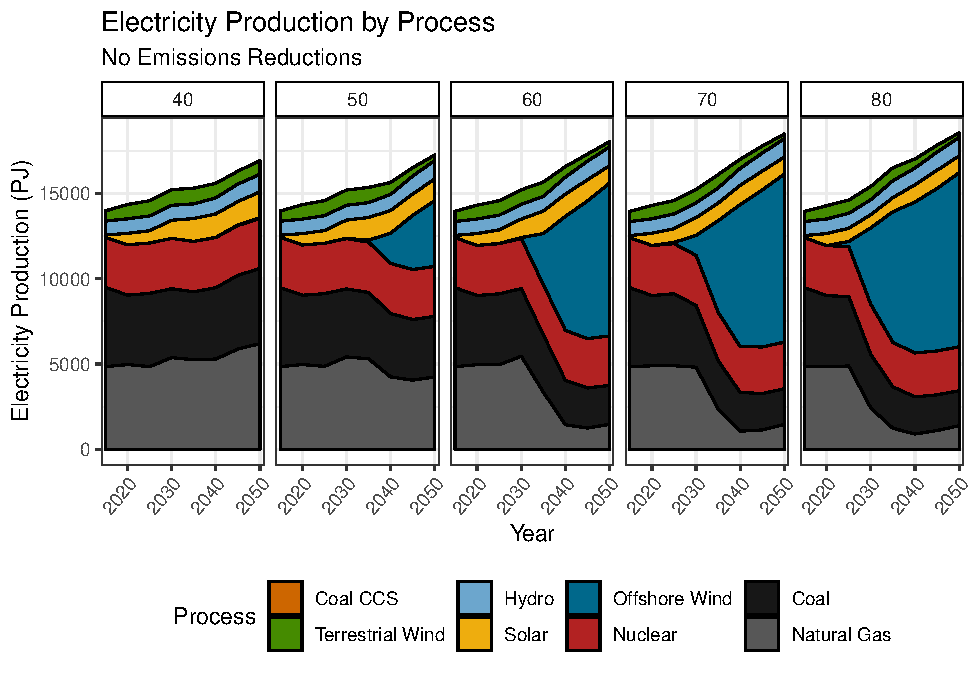
\includegraphics[width=0.5\linewidth]{osw_Report_files/figure-latex/unnamed-chunk-22-2}

\hypertarget{all-scenarios}{%
\subsection{All Scenarios}\label{all-scenarios}}

Complete Set

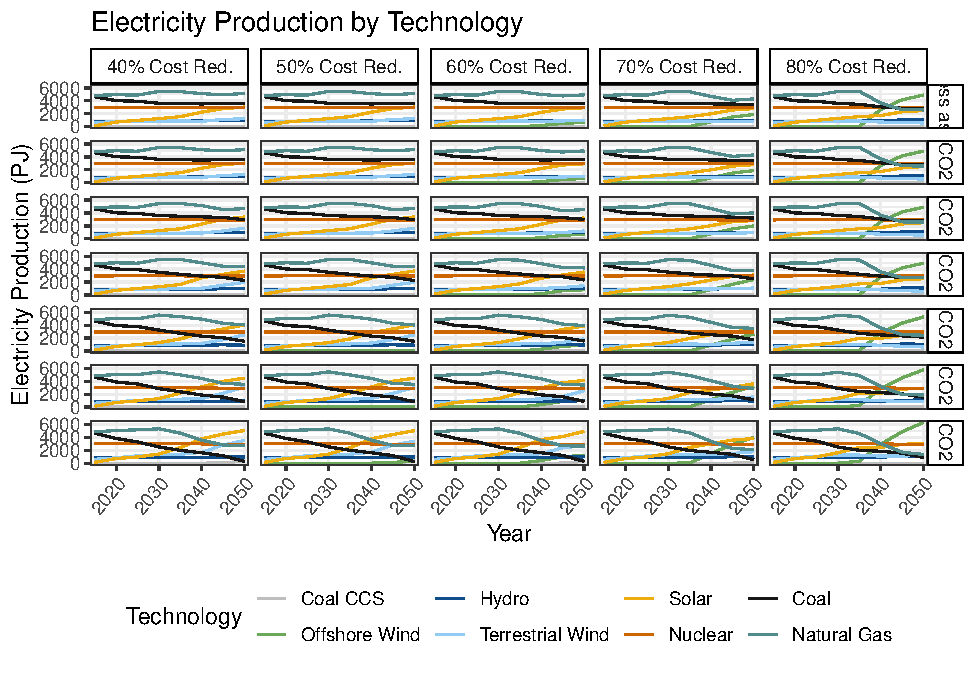
\includegraphics{osw_Report_files/figure-latex/unnamed-chunk-24-1.pdf}

Parsed Set

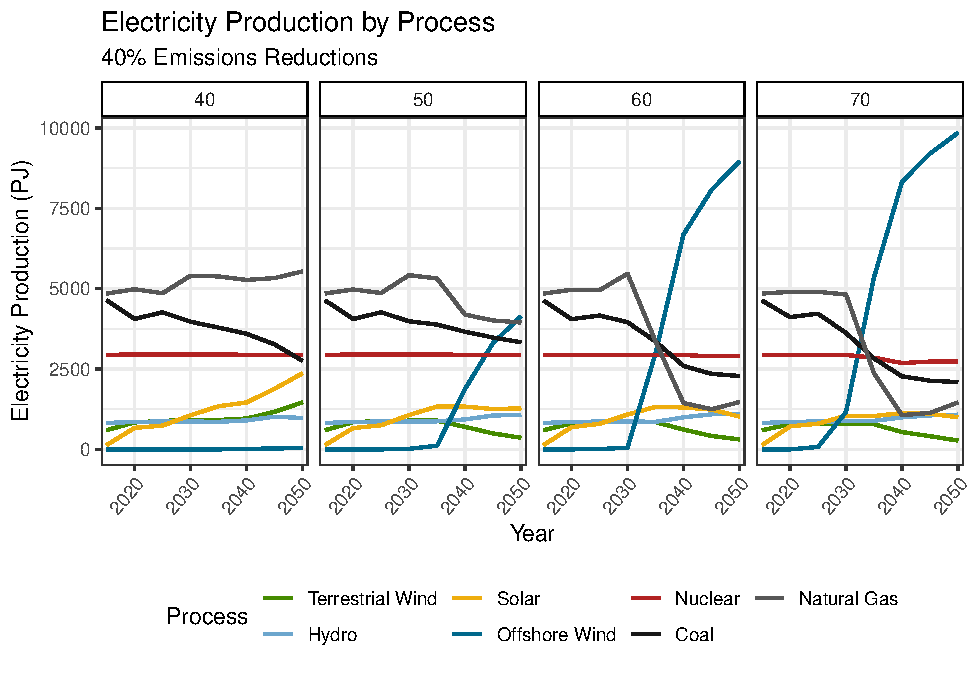
\includegraphics{osw_Report_files/figure-latex/unnamed-chunk-25-1.pdf}

\hypertarget{regional-mix}{%
\subsection{Regional Mix}\label{regional-mix}}

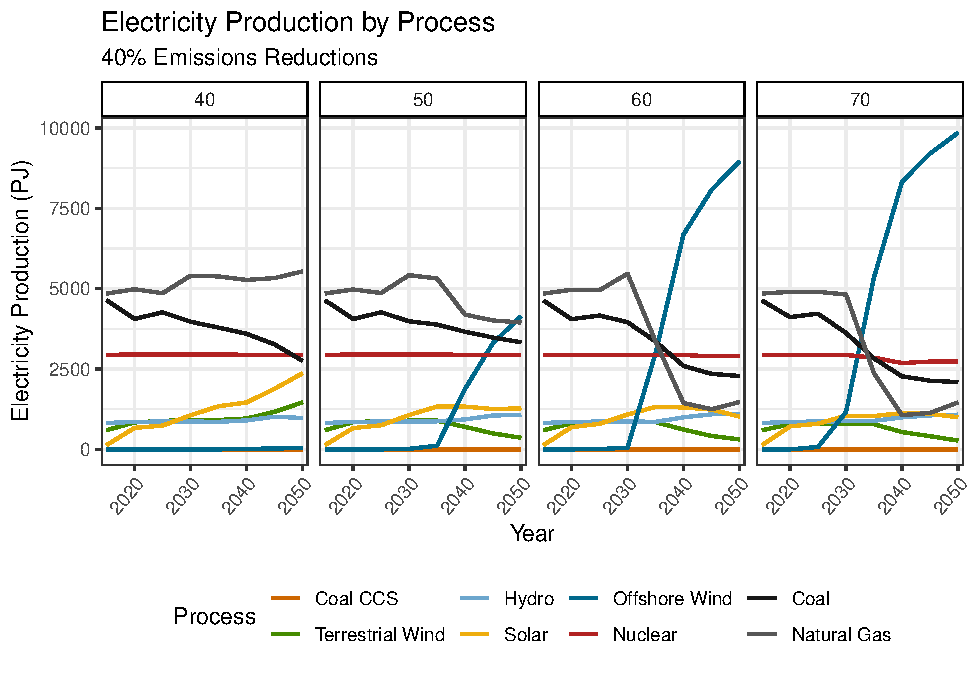
\includegraphics[width=0.5\linewidth]{osw_Report_files/figure-latex/unnamed-chunk-26-1}
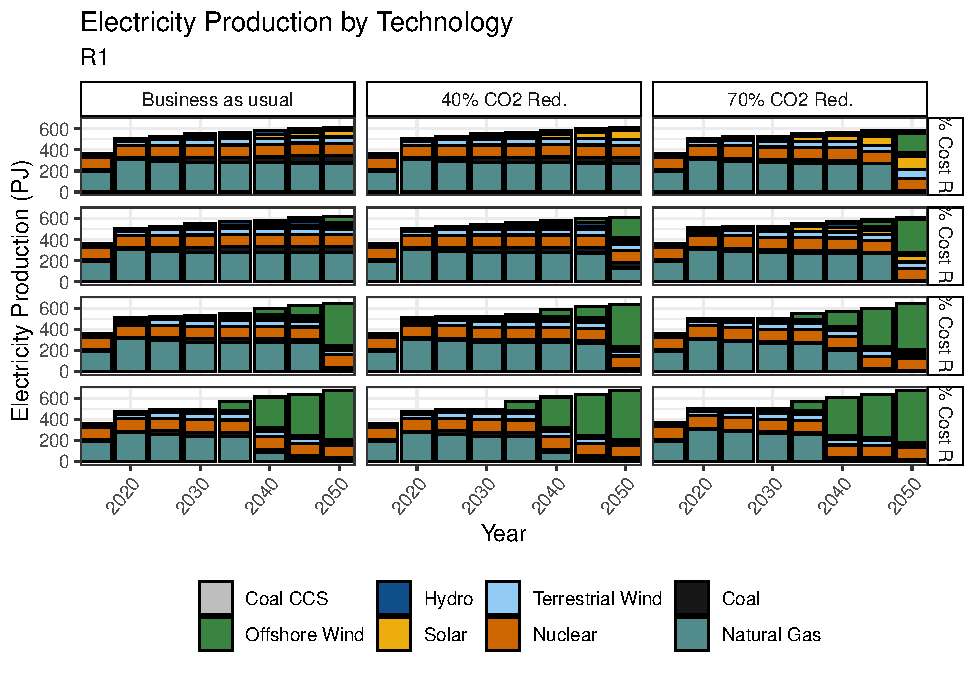
\includegraphics[width=0.5\linewidth]{osw_Report_files/figure-latex/unnamed-chunk-26-2}
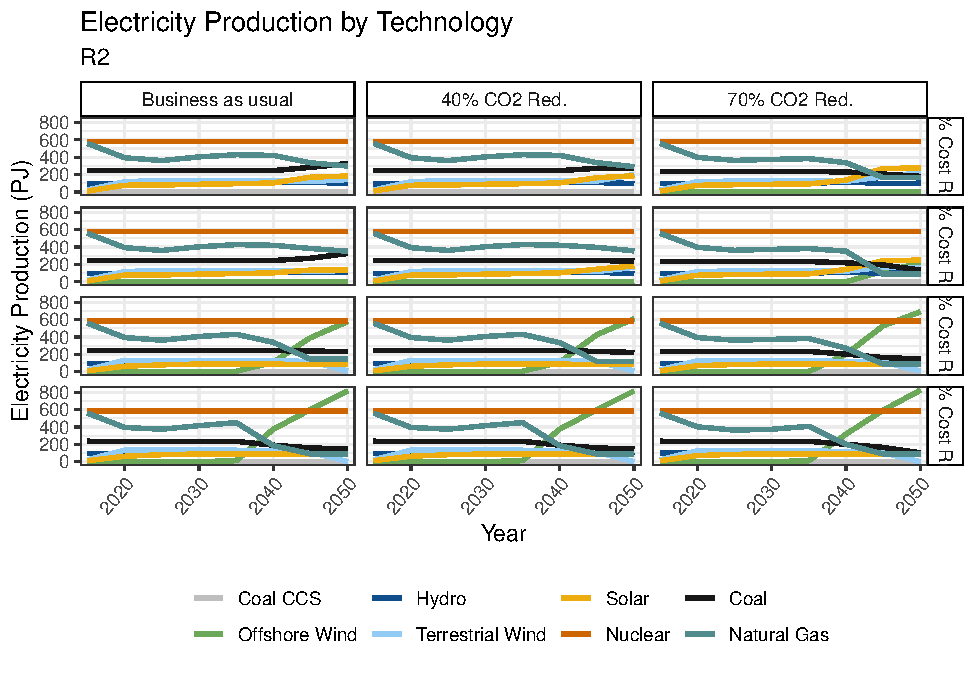
\includegraphics[width=0.5\linewidth]{osw_Report_files/figure-latex/unnamed-chunk-26-3}
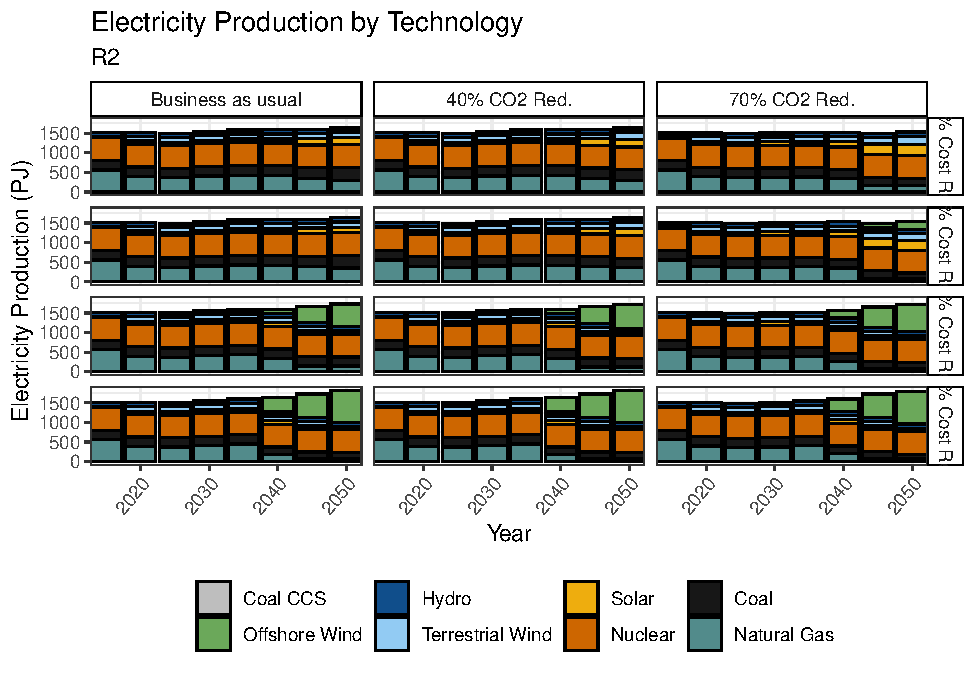
\includegraphics[width=0.5\linewidth]{osw_Report_files/figure-latex/unnamed-chunk-26-4}
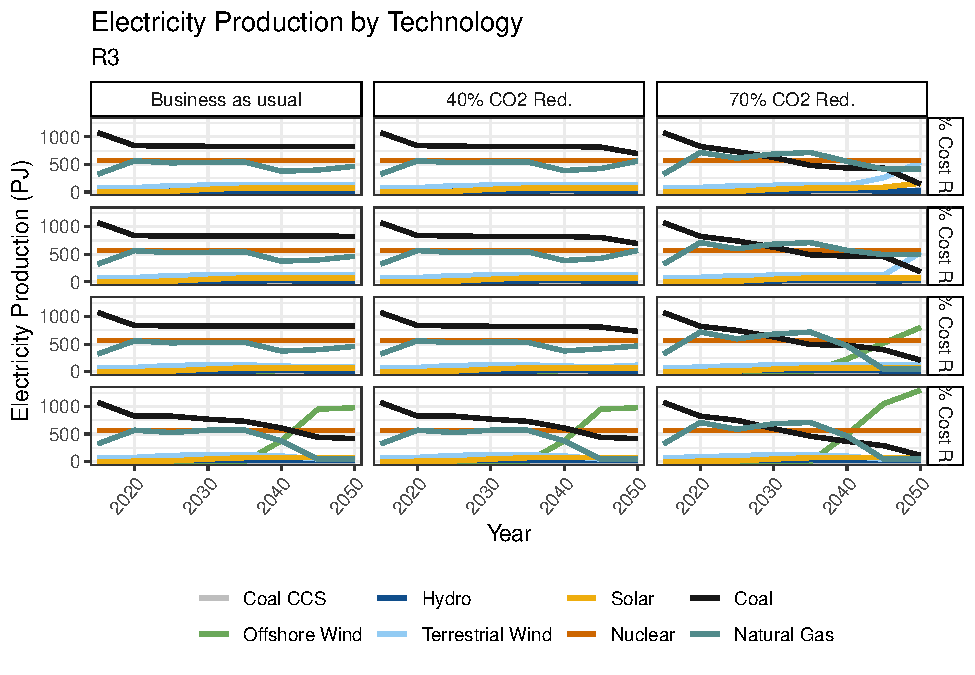
\includegraphics[width=0.5\linewidth]{osw_Report_files/figure-latex/unnamed-chunk-26-5}
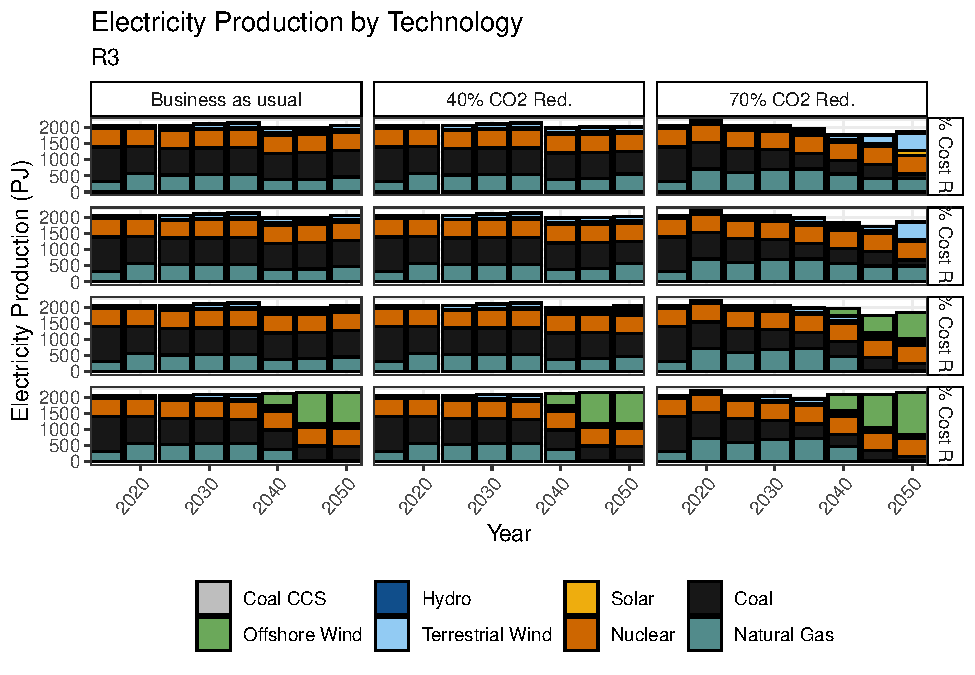
\includegraphics[width=0.5\linewidth]{osw_Report_files/figure-latex/unnamed-chunk-26-6}
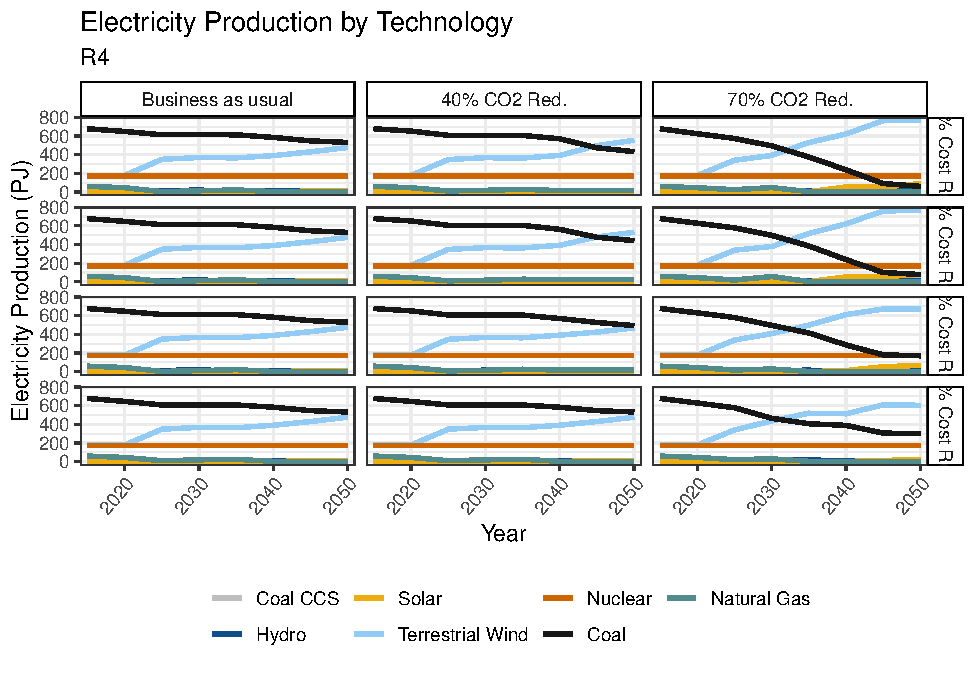
\includegraphics[width=0.5\linewidth]{osw_Report_files/figure-latex/unnamed-chunk-26-7}
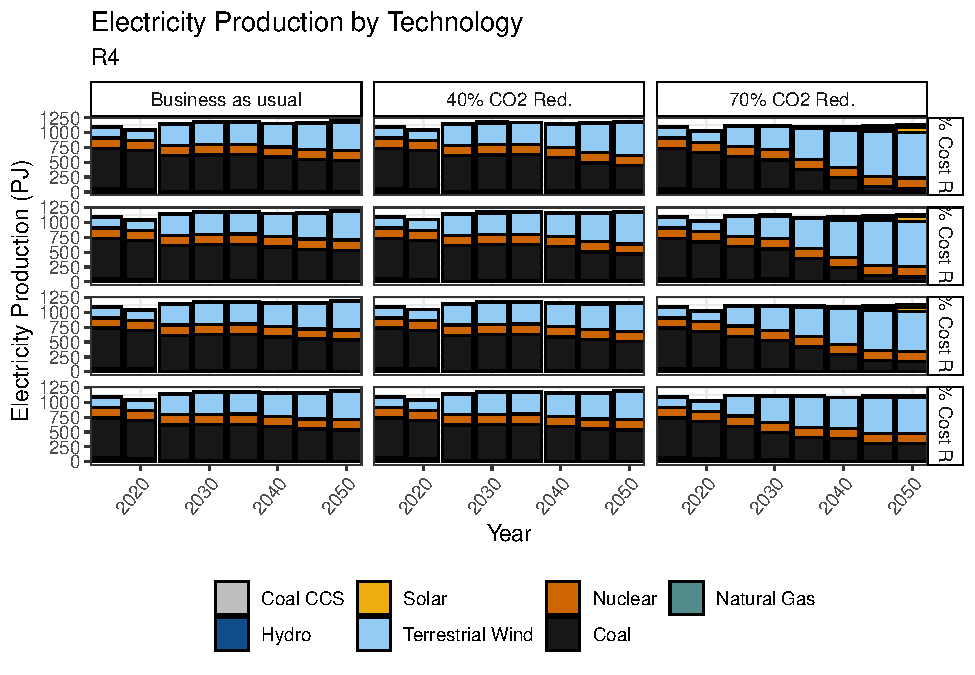
\includegraphics[width=0.5\linewidth]{osw_Report_files/figure-latex/unnamed-chunk-26-8}
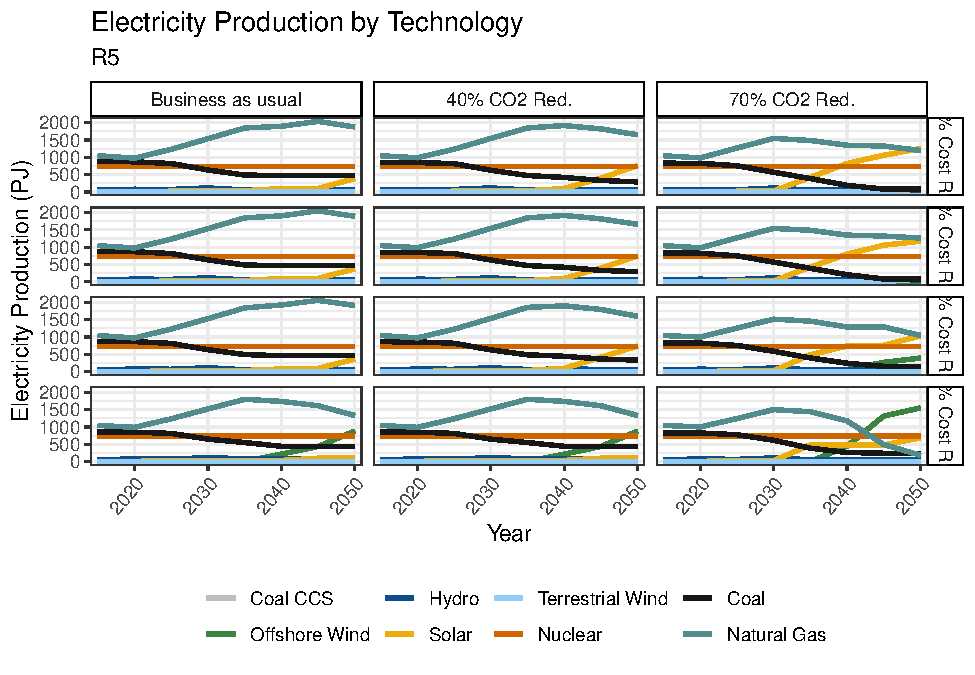
\includegraphics[width=0.5\linewidth]{osw_Report_files/figure-latex/unnamed-chunk-26-9}
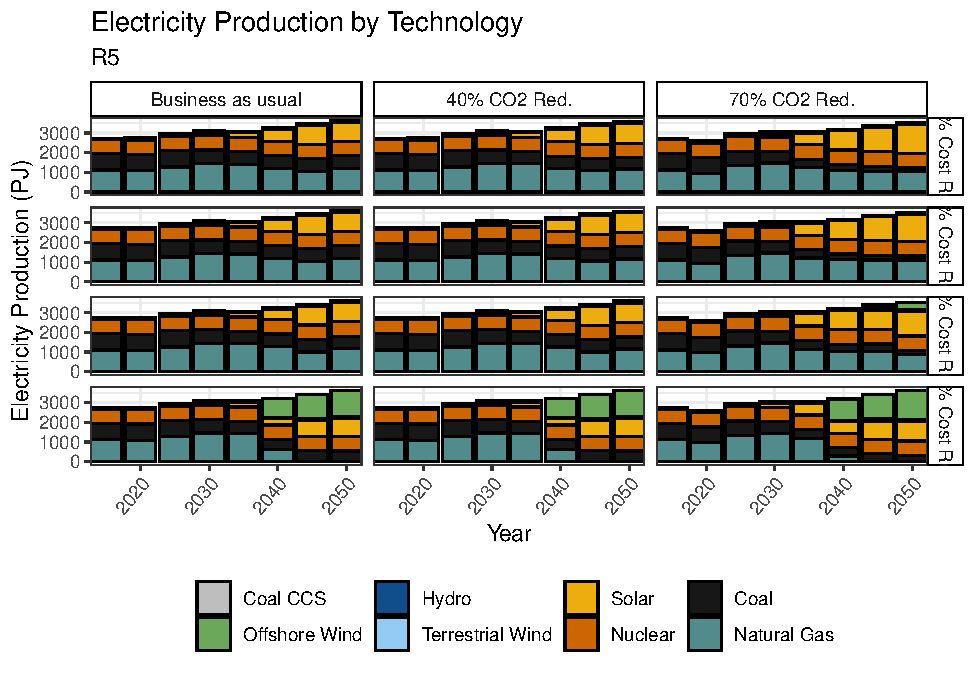
\includegraphics[width=0.5\linewidth]{osw_Report_files/figure-latex/unnamed-chunk-26-10}
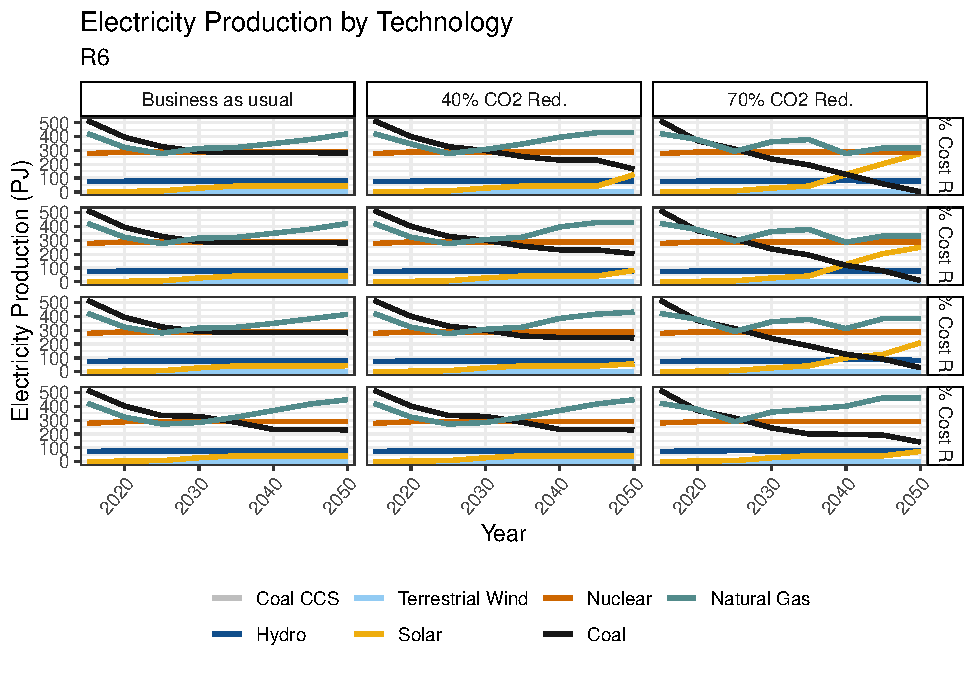
\includegraphics[width=0.5\linewidth]{osw_Report_files/figure-latex/unnamed-chunk-26-11}
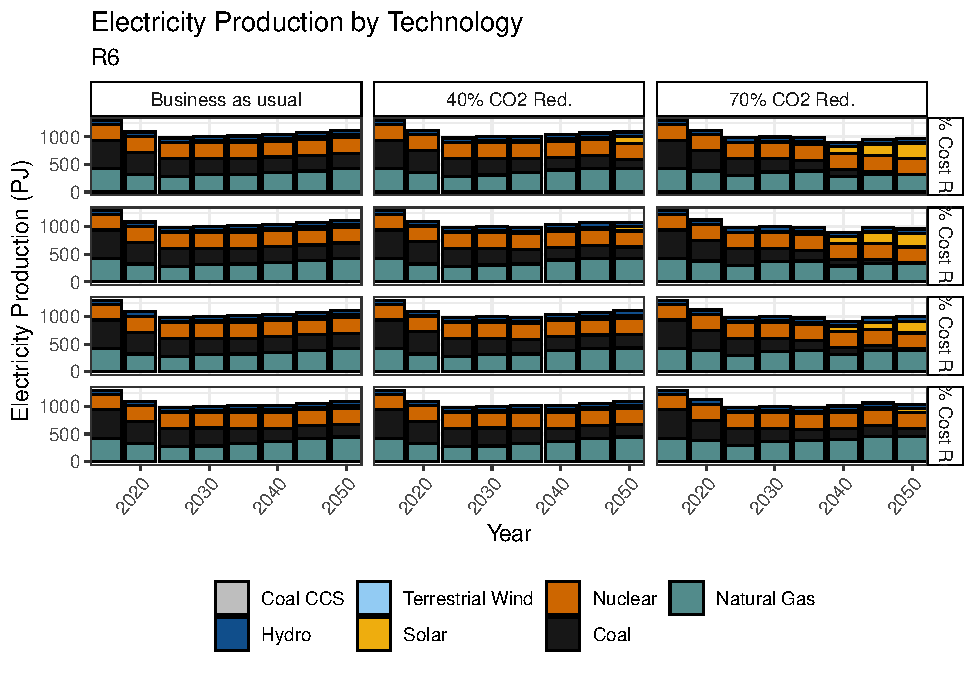
\includegraphics[width=0.5\linewidth]{osw_Report_files/figure-latex/unnamed-chunk-26-12}
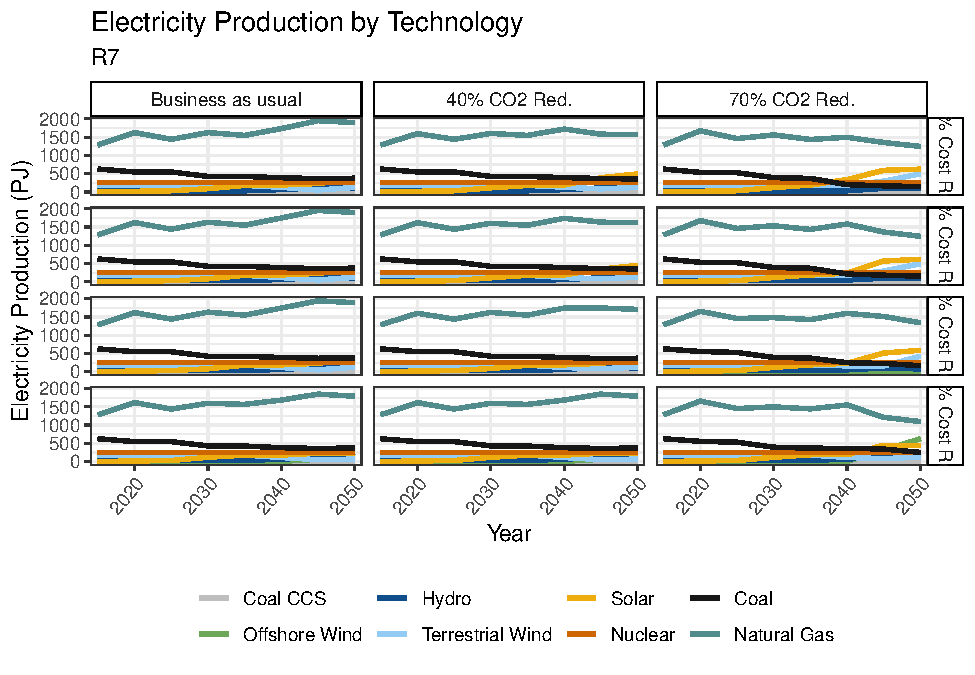
\includegraphics[width=0.5\linewidth]{osw_Report_files/figure-latex/unnamed-chunk-26-13}
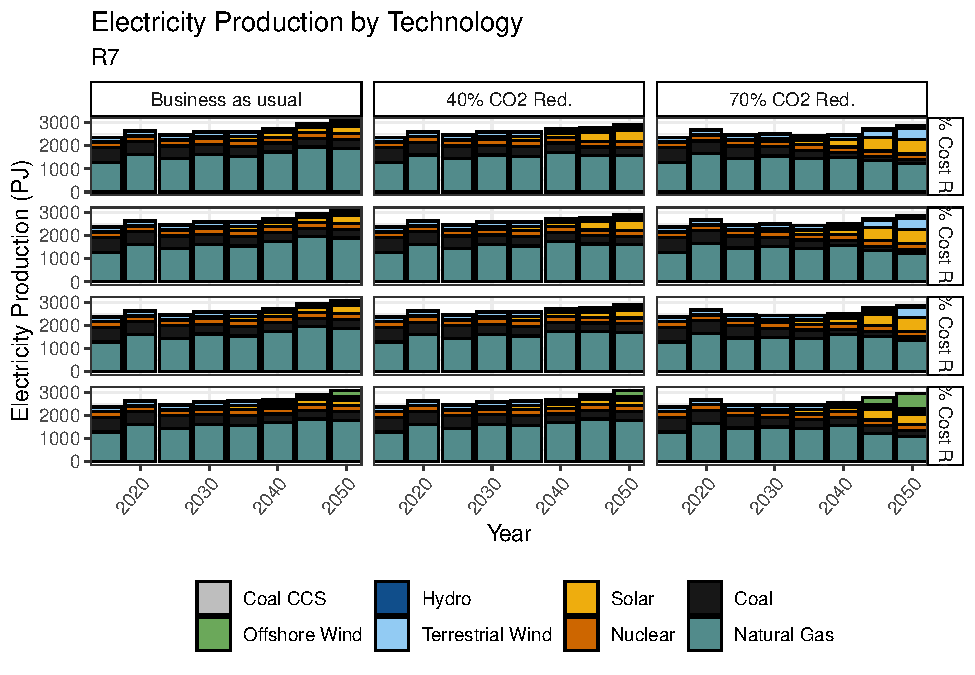
\includegraphics[width=0.5\linewidth]{osw_Report_files/figure-latex/unnamed-chunk-26-14}
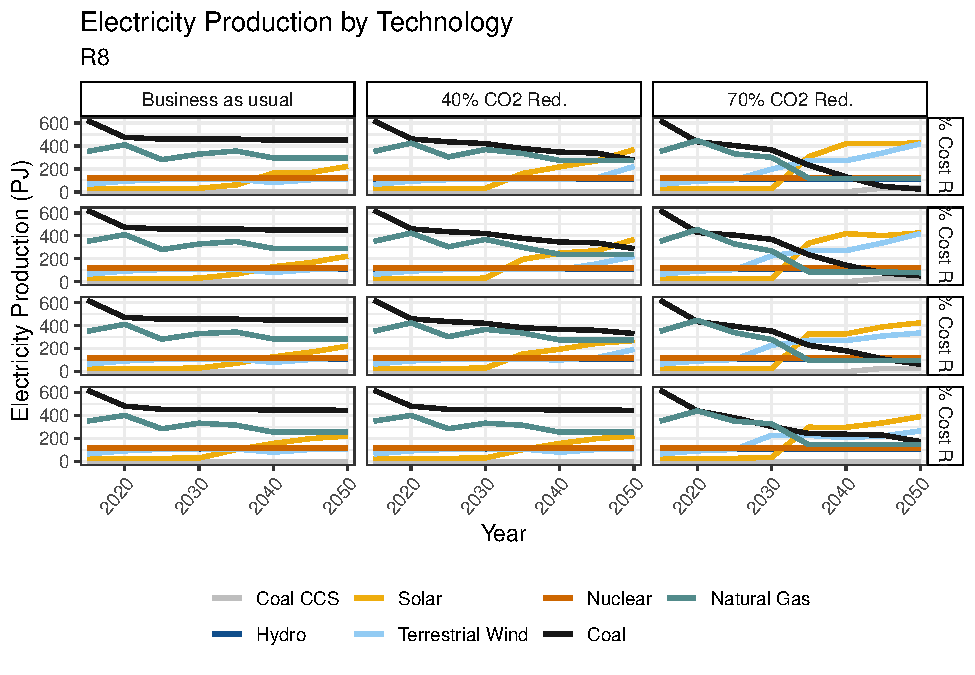
\includegraphics[width=0.5\linewidth]{osw_Report_files/figure-latex/unnamed-chunk-26-15}
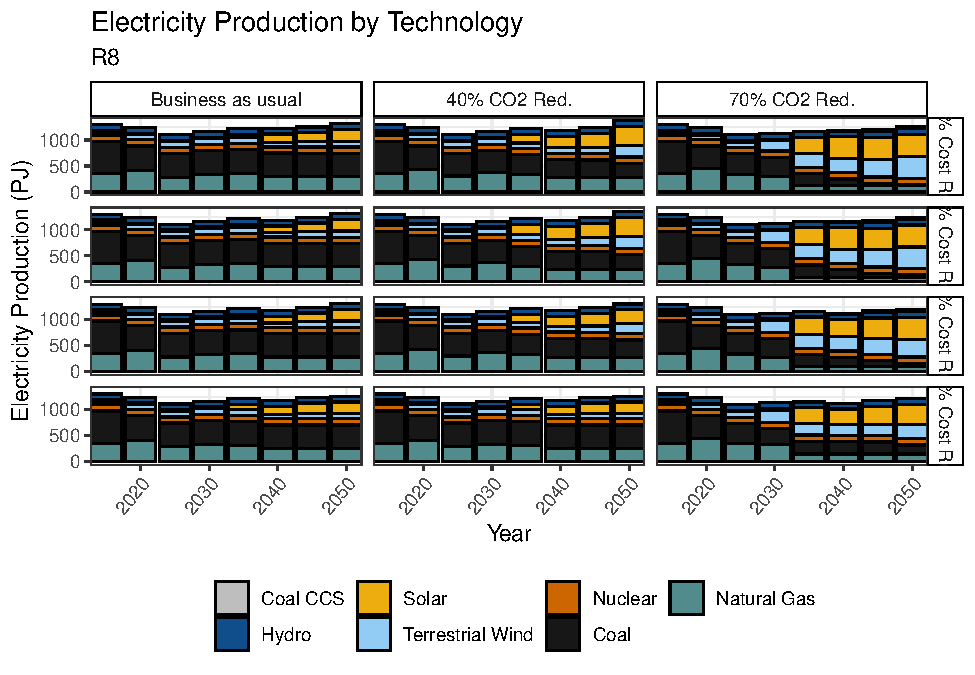
\includegraphics[width=0.5\linewidth]{osw_Report_files/figure-latex/unnamed-chunk-26-16}
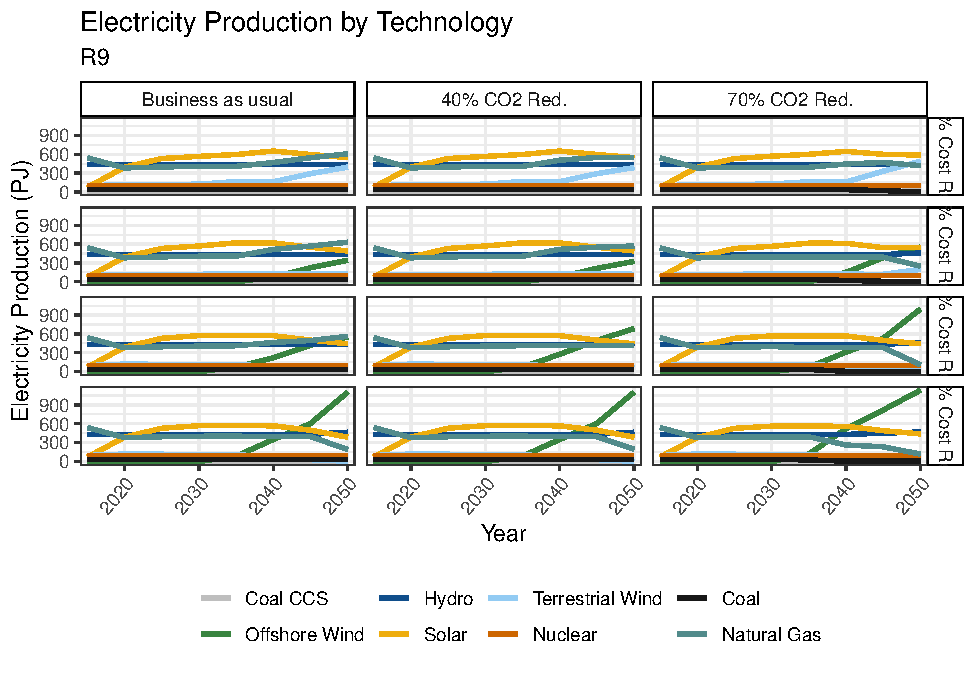
\includegraphics[width=0.5\linewidth]{osw_Report_files/figure-latex/unnamed-chunk-26-17}
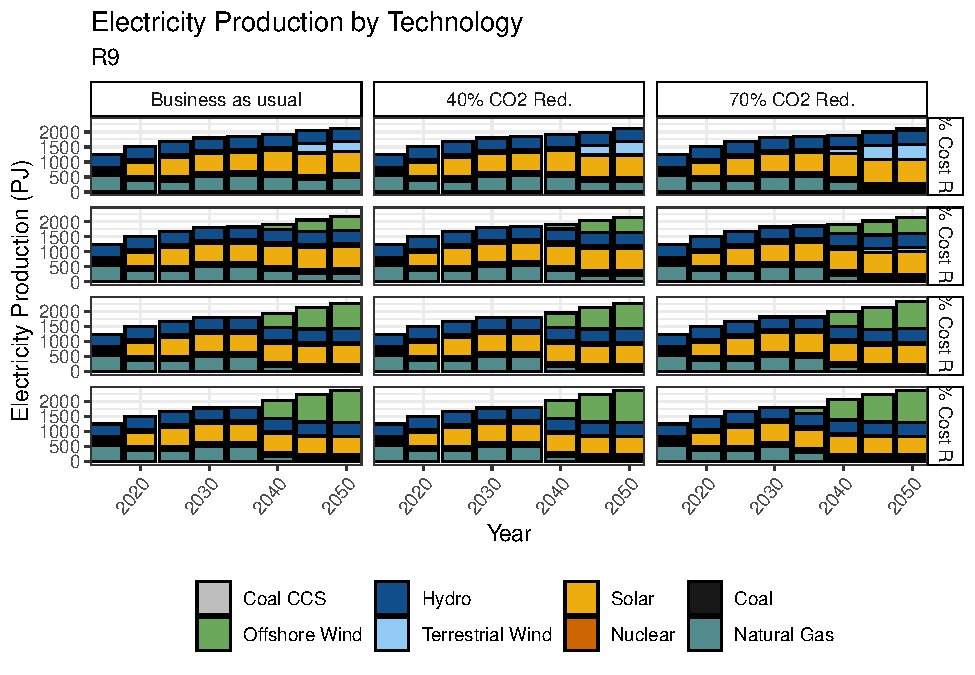
\includegraphics[width=0.5\linewidth]{osw_Report_files/figure-latex/unnamed-chunk-26-18}

\hypertarget{emissions-cap}{%
\subsection{Emissions Cap}\label{emissions-cap}}

BAU emissions

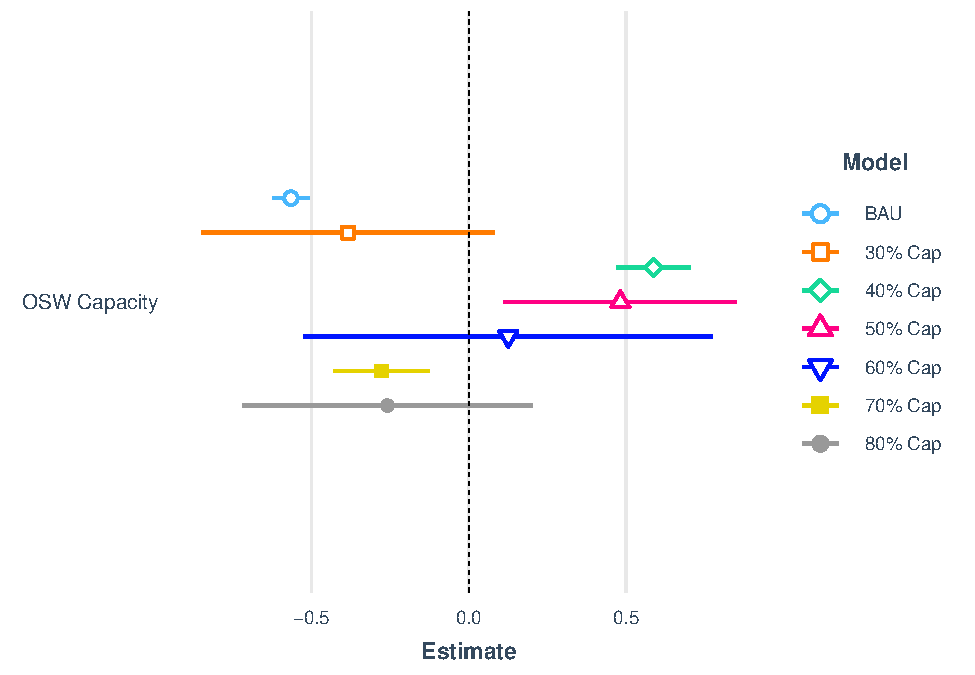
\includegraphics[width=0.5\linewidth]{osw_Report_files/figure-latex/unnamed-chunk-27-1}
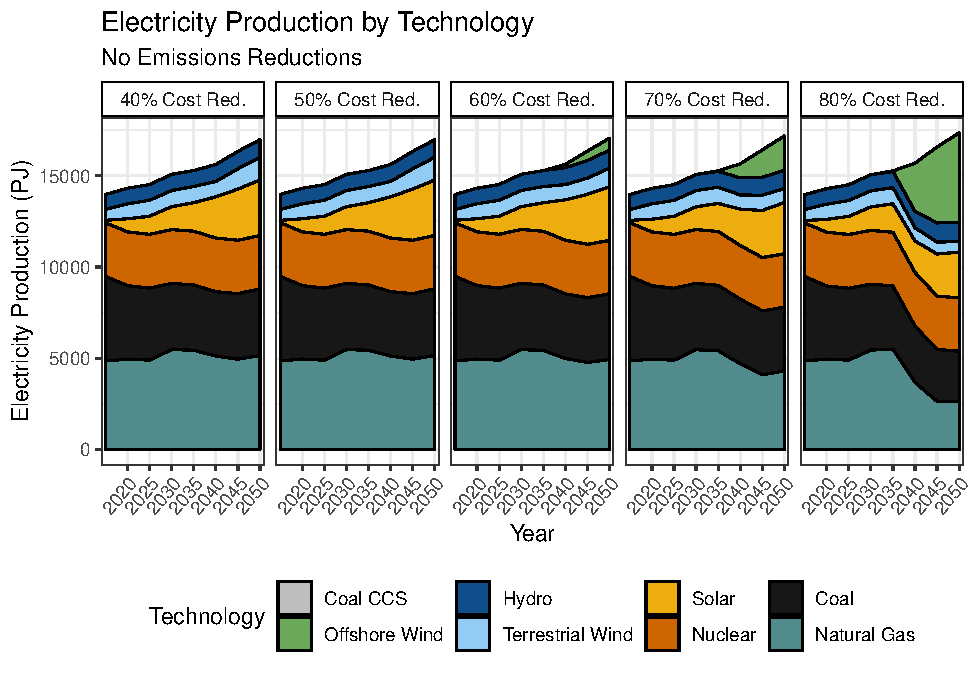
\includegraphics[width=0.5\linewidth]{osw_Report_files/figure-latex/unnamed-chunk-27-2}

30\% emissions reduction

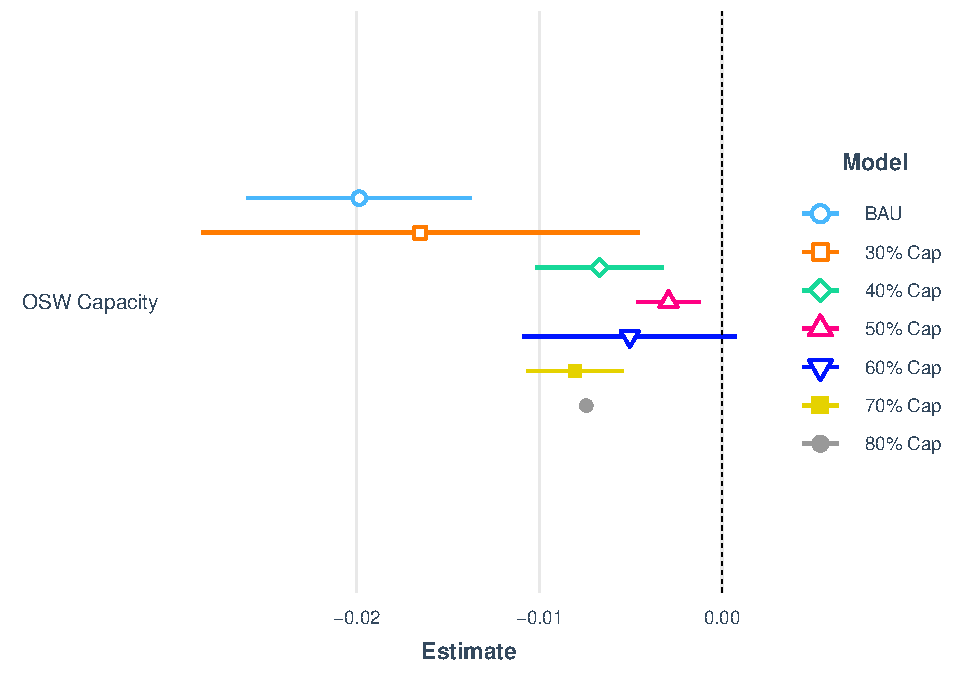
\includegraphics[width=0.5\linewidth]{osw_Report_files/figure-latex/unnamed-chunk-29-1}
\includegraphics[width=0.5\linewidth]{osw_Report_files/figure-latex/unnamed-chunk-29-2}

40\% emissions reduction

\includegraphics[width=0.5\linewidth]{osw_Report_files/figure-latex/unnamed-chunk-31-1}
\includegraphics[width=0.5\linewidth]{osw_Report_files/figure-latex/unnamed-chunk-31-2}

50\% emissions reduction

\includegraphics[width=0.5\linewidth]{osw_Report_files/figure-latex/unnamed-chunk-33-1}
\includegraphics[width=0.5\linewidth]{osw_Report_files/figure-latex/unnamed-chunk-33-2}

60\% emissions reduction

\includegraphics[width=0.5\linewidth]{osw_Report_files/figure-latex/unnamed-chunk-35-1}
\includegraphics[width=0.5\linewidth]{osw_Report_files/figure-latex/unnamed-chunk-35-2}

70\% emissions reduction

\includegraphics[width=0.5\linewidth]{osw_Report_files/figure-latex/unnamed-chunk-37-1}
\includegraphics[width=0.5\linewidth]{osw_Report_files/figure-latex/unnamed-chunk-37-2}

80\% emissions reduction

\includegraphics[width=0.5\linewidth]{osw_Report_files/figure-latex/unnamed-chunk-39-1}
\includegraphics[width=0.5\linewidth]{osw_Report_files/figure-latex/unnamed-chunk-39-2}

\hypertarget{cost-reductions}{%
\subsection{Cost Reductions}\label{cost-reductions}}

50\% cost reduction

\includegraphics[width=0.5\linewidth]{osw_Report_files/figure-latex/unnamed-chunk-41-1}
\includegraphics[width=0.5\linewidth]{osw_Report_files/figure-latex/unnamed-chunk-41-2}

60\% cost reduction

\includegraphics[width=0.5\linewidth]{osw_Report_files/figure-latex/unnamed-chunk-43-1}
\includegraphics[width=0.5\linewidth]{osw_Report_files/figure-latex/unnamed-chunk-43-2}

70\% cost reduction

\includegraphics[width=0.5\linewidth]{osw_Report_files/figure-latex/unnamed-chunk-45-1}
\includegraphics[width=0.5\linewidth]{osw_Report_files/figure-latex/unnamed-chunk-45-2}

80\% cost reduction

\includegraphics[width=0.5\linewidth]{osw_Report_files/figure-latex/unnamed-chunk-47-1}
\includegraphics[width=0.5\linewidth]{osw_Report_files/figure-latex/unnamed-chunk-47-2}

\hypertarget{heatmaps}{%
\subsection{Heatmaps}\label{heatmaps}}

\includegraphics{osw_Report_files/figure-latex/unnamed-chunk-49-1.pdf}

\includegraphics[width=0.5\linewidth]{osw_Report_files/figure-latex/unnamed-chunk-50-1}
\includegraphics[width=0.5\linewidth]{osw_Report_files/figure-latex/unnamed-chunk-50-2}
\includegraphics[width=0.5\linewidth]{osw_Report_files/figure-latex/unnamed-chunk-50-3}
\includegraphics[width=0.5\linewidth]{osw_Report_files/figure-latex/unnamed-chunk-50-4}
\includegraphics[width=0.5\linewidth]{osw_Report_files/figure-latex/unnamed-chunk-50-5}
\includegraphics[width=0.5\linewidth]{osw_Report_files/figure-latex/unnamed-chunk-50-6}
\includegraphics[width=0.5\linewidth]{osw_Report_files/figure-latex/unnamed-chunk-50-7}
\includegraphics[width=0.5\linewidth]{osw_Report_files/figure-latex/unnamed-chunk-50-8}

\hypertarget{market-share}{%
\subsection{Market Share}\label{market-share}}

\begin{verbatim}
## $Coal
##    Scenario         emred    costred  Technology            Year          
##  Length:336         BAU:48   20:56   Length:336         Length:336        
##  Class :character   30 :48   30: 0   Class :character   Class :character  
##  Mode  :character   40 :48   40:56   Mode  :character   Mode  :character  
##                     50 :48   50:56                                        
##                     60 :48   60:56                                        
##                     70 :48   70:56                                        
##                     80 :48   80:56                                        
##      Output           Total        MarketShare   
##  Min.   : 252.6   Min.   :13967   Min.   : 1.59  
##  1st Qu.:2748.5   1st Qu.:14323   1st Qu.:17.31  
##  Median :3540.3   Median :14993   Median :22.67  
##  Mean   :3271.2   Mean   :15060   Mean   :21.97  
##  3rd Qu.:3940.2   3rd Qu.:15621   3rd Qu.:27.18  
##  Max.   :4640.4   Max.   :17360   Max.   :33.19  
##                                                  
## 
## $`Coal CCS`
##    Scenario         emred    costred  Technology            Year          
##  Length:336         BAU:48   20:56   Length:336         Length:336        
##  Class :character   30 :48   30: 0   Class :character   Class :character  
##  Mode  :character   40 :48   40:56   Mode  :character   Mode  :character  
##                     50 :48   50:56                                        
##                     60 :48   60:56                                        
##                     70 :48   70:56                                        
##                     80 :48   80:56                                        
##      Output            Total        MarketShare     
##  Min.   :  0.000   Min.   :13967   Min.   :0.00000  
##  1st Qu.:  0.000   1st Qu.:14323   1st Qu.:0.00000  
##  Median :  0.000   Median :14993   Median :0.00000  
##  Mean   :  5.592   Mean   :15060   Mean   :0.03524  
##  3rd Qu.:  0.000   3rd Qu.:15621   3rd Qu.:0.00000  
##  Max.   :335.971   Max.   :17360   Max.   :2.13000  
##                                                     
## 
## $Hydro
##    Scenario         emred    costred  Technology            Year          
##  Length:336         BAU:48   20:56   Length:336         Length:336        
##  Class :character   30 :48   30: 0   Class :character   Class :character  
##  Mode  :character   40 :48   40:56   Mode  :character   Mode  :character  
##                     50 :48   50:56                                        
##                     60 :48   60:56                                        
##                     70 :48   70:56                                        
##                     80 :48   80:56                                        
##      Output           Total        MarketShare  
##  Min.   : 821.5   Min.   :13967   Min.   :5.64  
##  1st Qu.: 861.3   1st Qu.:14323   1st Qu.:5.88  
##  Median : 884.4   Median :14993   Median :5.95  
##  Mean   : 897.6   Mean   :15060   Mean   :5.96  
##  3rd Qu.: 930.0   3rd Qu.:15621   3rd Qu.:6.01  
##  Max.   :1112.8   Max.   :17360   Max.   :6.89  
##                                                 
## 
## $`Natural Gas`
##    Scenario         emred    costred  Technology            Year          
##  Length:336         BAU:48   20:56   Length:336         Length:336        
##  Class :character   30 :48   30: 0   Class :character   Class :character  
##  Mode  :character   40 :48   40:56   Mode  :character   Mode  :character  
##                     50 :48   50:56                                        
##                     60 :48   60:56                                        
##                     70 :48   70:56                                        
##                     80 :48   80:56                                        
##      Output         Total        MarketShare   
##  Min.   :1350   Min.   :13967   Min.   : 8.04  
##  1st Qu.:4595   1st Qu.:14323   1st Qu.:29.11  
##  Median :4923   Median :14993   Median :34.42  
##  Mean   :4689   Mean   :15060   Mean   :31.37  
##  3rd Qu.:5131   3rd Qu.:15621   3rd Qu.:35.23  
##  Max.   :5562   Max.   :17360   Max.   :37.10  
##                                                
## 
## $Nuclear
##    Scenario         emred    costred  Technology            Year          
##  Length:336         BAU:48   20:56   Length:336         Length:336        
##  Class :character   30 :48   30: 0   Class :character   Class :character  
##  Mode  :character   40 :48   40:56   Mode  :character   Mode  :character  
##                     50 :48   50:56                                        
##                     60 :48   60:56                                        
##                     70 :48   70:56                                        
##                     80 :48   80:56                                        
##      Output         Total        MarketShare   
##  Min.   :2927   Min.   :13967   Min.   :16.86  
##  1st Qu.:2935   1st Qu.:14323   1st Qu.:18.83  
##  Median :2951   Median :14993   Median :19.71  
##  Mean   :2954   Mean   :15060   Mean   :19.68  
##  3rd Qu.:2955   3rd Qu.:15621   3rd Qu.:20.64  
##  Max.   :3020   Max.   :17360   Max.   :21.43  
##                                                
## 
## $`Offshore Wind`
##    Scenario         emred    costred  Technology            Year          
##  Length:336         BAU:48   20:56   Length:336         Length:336        
##  Class :character   30 :48   30: 0   Class :character   Class :character  
##  Mode  :character   40 :48   40:56   Mode  :character   Mode  :character  
##                     50 :48   50:56                                        
##                     60 :48   60:56                                        
##                     70 :48   70:56                                        
##                     80 :48   80:56                                        
##      Output           Total        MarketShare    
##  Min.   :   0.0   Min.   :13967   Min.   : 0.000  
##  1st Qu.:   0.0   1st Qu.:14323   1st Qu.: 0.000  
##  Median :   0.0   Median :14993   Median : 0.000  
##  Mean   : 412.9   Mean   :15060   Mean   : 2.527  
##  3rd Qu.:   0.0   3rd Qu.:15621   3rd Qu.: 0.000  
##  Max.   :6285.8   Max.   :17360   Max.   :37.430  
##                                                   
## 
## $Solar
##    Scenario         emred    costred  Technology            Year          
##  Length:336         BAU:48   20:56   Length:336         Length:336        
##  Class :character   30 :48   30: 0   Class :character   Class :character  
##  Mode  :character   40 :48   40:56   Mode  :character   Mode  :character  
##                     50 :48   50:56                                        
##                     60 :48   60:56                                        
##                     70 :48   70:56                                        
##                     80 :48   80:56                                        
##      Output           Total        MarketShare    
##  Min.   : 133.3   Min.   :13967   Min.   : 0.950  
##  1st Qu.: 897.3   1st Qu.:14323   1st Qu.: 6.232  
##  Median :1541.6   Median :14993   Median :10.095  
##  Mean   :1767.7   Mean   :15060   Mean   :11.446  
##  3rd Qu.:2677.9   3rd Qu.:15621   3rd Qu.:16.920  
##  Max.   :5064.4   Max.   :17360   Max.   :32.180  
##                                                   
## 
## $`Terrestrial Wind`
##    Scenario         emred    costred  Technology            Year          
##  Length:336         BAU:48   20:56   Length:336         Length:336        
##  Class :character   30 :48   30: 0   Class :character   Class :character  
##  Mode  :character   40 :48   40:56   Mode  :character   Mode  :character  
##                     50 :48   50:56                                        
##                     60 :48   60:56                                        
##                     70 :48   70:56                                        
##                     80 :48   80:56                                        
##      Output           Total        MarketShare    
##  Min.   : 565.0   Min.   :13967   Min.   : 3.260  
##  1st Qu.: 825.2   1st Qu.:14323   1st Qu.: 5.720  
##  Median : 888.4   Median :14993   Median : 5.990  
##  Mean   :1062.2   Mean   :15060   Mean   : 7.015  
##  3rd Qu.:1181.4   3rd Qu.:15621   3rd Qu.: 7.595  
##  Max.   :3514.2   Max.   :17360   Max.   :22.330  
## 
\end{verbatim}

\begin{longtable}{>{\raggedright\arraybackslash}p{2 cm}lrrrrrr}
\caption{\label{tab:unnamed-chunk-3}2050 Percent Market Share by Technology}\\
\toprule
\multicolumn{2}{c}{ } & \multicolumn{6}{c}{Cost Reduction (\%)} \\
\cmidrule(l{3pt}r{3pt}){3-8}
Technology & CO2 Cap & 20 & 40 & 50 & 60 & 70 & 80\\
\midrule
\rowcolor{gray!6}   & BAU & 21.5 & 21.5 & 21.5 & 21.1 & 20.3 & 16.0\\

 & 30 & 21.4 & 21.4 & 21.4 & 21.1 & 20.3 & 16.0\\

\rowcolor{gray!6}   & 40 & 17.9 & 17.9 & 17.9 & 18.2 & 19.0 & 16.0\\

 & 50 & 13.9 & 13.9 & 13.9 & 14.3 & 14.9 & 15.5\\

\rowcolor{gray!6}   & 60 & 9.4 & 9.4 & 9.4 & 9.7 & 10.5 & 12.6\\

 & 70 & 5.2 & 5.2 & 5.2 & 5.5 & 6.9 & 9.1\\

\rowcolor{gray!6}  \multirow{-7}{2 cm}{\raggedright\arraybackslash Coal} & 80 & 1.6 & 1.6 & 1.6 & 1.7 & 3.4 & 5.3\\
\cmidrule{1-8}
 & BAU & 0.0 & 0.0 & 0.0 & 0.0 & 0.0 & 0.0\\

\rowcolor{gray!6}   & 30 & 0.0 & 0.0 & 0.0 & 0.0 & 0.0 & 0.0\\

 & 40 & 0.0 & 0.0 & 0.0 & 0.0 & 0.0 & 0.0\\

\rowcolor{gray!6}   & 50 & 0.0 & 0.0 & 0.0 & 0.0 & 0.0 & 0.0\\

 & 60 & 0.0 & 0.0 & 0.0 & 0.0 & 0.0 & 0.0\\

\rowcolor{gray!6}   & 70 & 0.6 & 0.6 & 0.6 & 0.4 & 0.0 & 0.0\\

\multirow{-7}{2 cm}{\raggedright\arraybackslash Coal CCS} & 80 & 2.1 & 2.1 & 2.1 & 1.8 & 0.8 & 0.0\\
\cmidrule{1-8}
\rowcolor{gray!6}   & BAU & 5.7 & 5.7 & 5.7 & 5.8 & 5.8 & 6.1\\

 & 30 & 5.6 & 5.6 & 5.6 & 5.8 & 5.8 & 6.1\\

\rowcolor{gray!6}   & 40 & 5.7 & 5.7 & 5.7 & 5.9 & 5.9 & 6.1\\

 & 50 & 5.8 & 5.8 & 5.8 & 6.0 & 5.9 & 6.1\\

\rowcolor{gray!6}   & 60 & 5.7 & 5.7 & 5.7 & 5.8 & 5.8 & 6.2\\

 & 70 & 6.0 & 6.0 & 6.0 & 6.0 & 5.8 & 6.4\\

\rowcolor{gray!6}  \multirow{-7}{2 cm}{\raggedright\arraybackslash Hydro} & 80 & 6.0 & 6.0 & 6.0 & 6.1 & 6.0 & 6.2\\
\cmidrule{1-8}
 & BAU & 30.3 & 30.3 & 30.3 & 28.9 & 25.0 & 15.0\\

\rowcolor{gray!6}   & 30 & 30.2 & 30.2 & 30.2 & 28.9 & 25.1 & 15.0\\

 & 40 & 28.3 & 28.3 & 28.3 & 27.2 & 23.7 & 15.0\\

\rowcolor{gray!6}   & 50 & 27.1 & 27.1 & 27.1 & 25.9 & 22.5 & 15.4\\

 & 60 & 25.3 & 25.3 & 25.3 & 24.6 & 21.4 & 14.3\\

\rowcolor{gray!6}   & 70 & 22.2 & 22.2 & 22.2 & 21.4 & 17.6 & 11.0\\

\multirow{-7}{2 cm}{\raggedright\arraybackslash Natural Gas} & 80 & 17.1 & 17.1 & 16.9 & 16.6 & 12.8 & 8.0\\
\cmidrule{1-8}
\rowcolor{gray!6}   & BAU & 17.2 & 17.2 & 17.2 & 17.1 & 17.0 & 16.9\\

 & 30 & 17.2 & 17.2 & 17.2 & 17.1 & 17.0 & 16.9\\

\rowcolor{gray!6}   & 40 & 17.7 & 17.7 & 17.7 & 17.6 & 17.3 & 16.9\\

 & 50 & 18.2 & 18.2 & 18.2 & 18.1 & 17.5 & 16.9\\

\rowcolor{gray!6}   & 60 & 18.3 & 18.3 & 18.3 & 18.3 & 17.8 & 17.1\\

 & 70 & 18.4 & 18.4 & 18.4 & 18.3 & 18.0 & 17.3\\

\rowcolor{gray!6}  \multirow{-7}{2 cm}{\raggedright\arraybackslash Nuclear} & 80 & 18.6 & 18.6 & 18.4 & 18.3 & 18.0 & 17.4\\
\cmidrule{1-8}
 & BAU & 0.0 & 0.0 & 0.0 & 3.9 & 10.9 & 28.2\\

\rowcolor{gray!6}   & 30 & 0.0 & 0.0 & 0.0 & 3.9 & 10.9 & 28.2\\

 & 40 & 0.0 & 0.0 & 0.0 & 4.2 & 11.8 & 28.2\\

\rowcolor{gray!6}   & 50 & 0.0 & 0.0 & 0.0 & 4.9 & 14.3 & 28.3\\

 & 60 & 0.0 & 0.0 & 0.2 & 5.7 & 16.1 & 30.8\\

\rowcolor{gray!6}   & 70 & 0.0 & 0.0 & 0.7 & 6.8 & 19.8 & 34.0\\

\multirow{-7}{2 cm}{\raggedright\arraybackslash Offshore Wind} & 80 & 0.0 & 0.0 & 1.8 & 7.8 & 24.6 & 37.4\\
\cmidrule{1-8}
\rowcolor{gray!6}   & BAU & 17.9 & 17.9 & 17.9 & 17.2 & 16.3 & 14.4\\

 & 30 & 18.0 & 18.0 & 18.0 & 17.2 & 16.3 & 14.4\\

\rowcolor{gray!6}   & 40 & 20.5 & 20.5 & 20.5 & 19.4 & 16.7 & 14.4\\

 & 50 & 22.9 & 22.9 & 22.9 & 21.9 & 18.5 & 14.5\\

\rowcolor{gray!6}   & 60 & 25.4 & 25.4 & 25.4 & 24.1 & 20.2 & 15.2\\

 & 70 & 28.1 & 28.1 & 28.0 & 25.9 & 22.2 & 17.2\\

\rowcolor{gray!6}  \multirow{-7}{2 cm}{\raggedright\arraybackslash Solar} & 80 & 32.2 & 32.2 & 31.7 & 30.8 & 23.4 & 18.4\\
\cmidrule{1-8}
 & BAU & 7.3 & 7.3 & 7.3 & 6.0 & 4.5 & 3.4\\

\rowcolor{gray!6}   & 30 & 7.5 & 7.5 & 7.5 & 6.0 & 4.5 & 3.4\\

 & 40 & 9.9 & 9.9 & 9.9 & 7.4 & 5.6 & 3.4\\

\rowcolor{gray!6}   & 50 & 12.1 & 12.1 & 12.1 & 8.8 & 6.4 & 3.3\\

 & 60 & 15.8 & 15.8 & 15.6 & 11.8 & 8.3 & 3.7\\

\rowcolor{gray!6}   & 70 & 19.6 & 19.6 & 19.0 & 15.8 & 9.7 & 5.0\\

\multirow{-7}{2 cm}{\raggedright\arraybackslash Terrestrial Wind} & 80 & 22.3 & 22.3 & 21.3 & 17.0 & 10.9 & 7.2\\
\bottomrule
\end{longtable}

\hypertarget{renewable-contributions}{%
\subsection{Renewable Contributions}\label{renewable-contributions}}

\includegraphics{osw_Report_files/figure-latex/unnamed-chunk-53-1.pdf}

\hypertarget{retirements-and-additions}{%
\subsection{Retirements and Additions}\label{retirements-and-additions}}

Basecase year-on-year changes in the grid mix. Shows the modeled
fluctuations in generation. All following quantifications of grid mix
changes are as compared to these changes in the basecase.

\includegraphics{osw_Report_files/figure-latex/unnamed-chunk-54-1.pdf}

\hypertarget{changes-over-baseline}{%
\subsection{Changes Over Baseline}\label{changes-over-baseline}}

Summary Graph

\includegraphics{osw_Report_files/figure-latex/unnamed-chunk-55-1.pdf}
\includegraphics{osw_Report_files/figure-latex/unnamed-chunk-56-1.pdf}

Regional Summary Graphs

\includegraphics{osw_Report_files/figure-latex/unnamed-chunk-57-1.pdf}
\includegraphics{osw_Report_files/figure-latex/unnamed-chunk-57-2.pdf}
\includegraphics{osw_Report_files/figure-latex/unnamed-chunk-57-3.pdf}
\includegraphics{osw_Report_files/figure-latex/unnamed-chunk-57-4.pdf}
\includegraphics{osw_Report_files/figure-latex/unnamed-chunk-57-5.pdf}
\includegraphics{osw_Report_files/figure-latex/unnamed-chunk-57-6.pdf}
\includegraphics{osw_Report_files/figure-latex/unnamed-chunk-57-7.pdf}
\includegraphics{osw_Report_files/figure-latex/unnamed-chunk-57-8.pdf}
\includegraphics{osw_Report_files/figure-latex/unnamed-chunk-57-9.pdf}

By Emissions Reduction \%

\includegraphics[width=0.5\linewidth]{osw_Report_files/figure-latex/unnamed-chunk-58-1}
\includegraphics[width=0.5\linewidth]{osw_Report_files/figure-latex/unnamed-chunk-58-2}
\includegraphics[width=0.5\linewidth]{osw_Report_files/figure-latex/unnamed-chunk-58-3}
\includegraphics[width=0.5\linewidth]{osw_Report_files/figure-latex/unnamed-chunk-58-4}
\includegraphics[width=0.5\linewidth]{osw_Report_files/figure-latex/unnamed-chunk-58-5}
\includegraphics[width=0.5\linewidth]{osw_Report_files/figure-latex/unnamed-chunk-58-6}
\includegraphics[width=0.5\linewidth]{osw_Report_files/figure-latex/unnamed-chunk-58-7}

By Cost Reduction \%

\includegraphics[width=0.5\linewidth]{osw_Report_files/figure-latex/unnamed-chunk-59-1}
\includegraphics[width=0.5\linewidth]{osw_Report_files/figure-latex/unnamed-chunk-59-2}
\includegraphics[width=0.5\linewidth]{osw_Report_files/figure-latex/unnamed-chunk-59-3}
\includegraphics[width=0.5\linewidth]{osw_Report_files/figure-latex/unnamed-chunk-59-4}
\includegraphics[width=0.5\linewidth]{osw_Report_files/figure-latex/unnamed-chunk-59-5}

\hypertarget{emissions}{%
\section{Emissions}\label{emissions}}

\hypertarget{baseline}{%
\subsection{Baseline}\label{baseline}}

\includegraphics[width=0.5\linewidth]{osw_Report_files/figure-latex/unnamed-chunk-60-1}
\includegraphics[width=0.5\linewidth]{osw_Report_files/figure-latex/unnamed-chunk-60-2}

\hypertarget{emissions-by-scenario-and-commodity}{%
\subsection{Emissions by Scenario and
Commodity}\label{emissions-by-scenario-and-commodity}}

\includegraphics[width=0.5\linewidth]{osw_Report_files/figure-latex/unnamed-chunk-61-1}
\includegraphics[width=0.5\linewidth]{osw_Report_files/figure-latex/unnamed-chunk-61-2}

\hypertarget{emissions-by-commodity---values}{%
\subsection{Emissions by Commodity -
Values}\label{emissions-by-commodity---values}}

\includegraphics[width=0.5\linewidth]{osw_Report_files/figure-latex/unnamed-chunk-62-1}
\includegraphics[width=0.5\linewidth]{osw_Report_files/figure-latex/unnamed-chunk-62-2}
\includegraphics[width=0.5\linewidth]{osw_Report_files/figure-latex/unnamed-chunk-62-3}
\includegraphics[width=0.5\linewidth]{osw_Report_files/figure-latex/unnamed-chunk-62-4}
\includegraphics[width=0.5\linewidth]{osw_Report_files/figure-latex/unnamed-chunk-62-5}
\includegraphics[width=0.5\linewidth]{osw_Report_files/figure-latex/unnamed-chunk-62-6}
\includegraphics[width=0.5\linewidth]{osw_Report_files/figure-latex/unnamed-chunk-62-7}
\includegraphics[width=0.5\linewidth]{osw_Report_files/figure-latex/unnamed-chunk-62-8}
\includegraphics[width=0.5\linewidth]{osw_Report_files/figure-latex/unnamed-chunk-62-9}
\includegraphics[width=0.5\linewidth]{osw_Report_files/figure-latex/unnamed-chunk-62-10}

\hypertarget{emissions-by-commodity---percent-reduction}{%
\subsection{Emissions by Commodity - Percent
Reduction}\label{emissions-by-commodity---percent-reduction}}

\includegraphics[width=0.5\linewidth]{osw_Report_files/figure-latex/unnamed-chunk-63-1}
\includegraphics[width=0.5\linewidth]{osw_Report_files/figure-latex/unnamed-chunk-63-2}
\includegraphics[width=0.5\linewidth]{osw_Report_files/figure-latex/unnamed-chunk-63-3}
\includegraphics[width=0.5\linewidth]{osw_Report_files/figure-latex/unnamed-chunk-63-4}
\includegraphics[width=0.5\linewidth]{osw_Report_files/figure-latex/unnamed-chunk-63-5}

\hypertarget{total-electricity-production}{%
\section{Total Electricity
Production}\label{total-electricity-production}}

\includegraphics[width=0.5\linewidth]{osw_Report_files/figure-latex/unnamed-chunk-64-1}
\includegraphics[width=0.5\linewidth]{osw_Report_files/figure-latex/unnamed-chunk-64-2}

\hypertarget{correlations}{%
\section{Correlations}\label{correlations}}

\includegraphics{osw_Report_files/figure-latex/unnamed-chunk-65-1.pdf}

\hypertarget{regressions}{%
\section{Regressions}\label{regressions}}

 
  \providecommand{\huxb}[2]{\arrayrulecolor[RGB]{#1}\global\arrayrulewidth=#2pt}
  \providecommand{\huxvb}[2]{\color[RGB]{#1}\vrule width #2pt}
  \providecommand{\huxtpad}[1]{\rule{0pt}{\baselineskip+#1}}
  \providecommand{\huxbpad}[1]{\rule[-#1]{0pt}{#1}}

\begin{table}[h]
\centering
\begin{threeparttable}
\begin{tabularx}{0.5\textwidth}{p{0.125\textwidth} p{0.125\textwidth} p{0.125\textwidth} p{0.125\textwidth}}


\hhline{>{\huxb{0, 0, 0}{0.8}}->{\huxb{0, 0, 0}{0.8}}->{\huxb{0, 0, 0}{0.8}}->{\huxb{0, 0, 0}{0.8}}-}
\arrayrulecolor{black}

\multicolumn{1}{!{\huxvb{0, 0, 0}{0}}c!{\huxvb{0, 0, 0}{0}}}{\huxtpad{4pt}\centering \huxbpad{4pt}} &
\multicolumn{1}{c!{\huxvb{0, 0, 0}{0}}}{\huxtpad{4pt}\centering OSW Capacity\huxbpad{4pt}} &
\multicolumn{1}{c!{\huxvb{0, 0, 0}{0}}}{\huxtpad{4pt}\centering \% Renewables\huxbpad{4pt}} &
\multicolumn{1}{c!{\huxvb{0, 0, 0}{0}}}{\huxtpad{4pt}\centering Total Elc\huxbpad{4pt}} \tabularnewline[-0.5pt]


\hhline{>{\huxb{255, 255, 255}{0.4}}->{\huxb{0, 0, 0}{0.4}}->{\huxb{0, 0, 0}{0.4}}->{\huxb{0, 0, 0}{0.4}}-}
\arrayrulecolor{black}

\multicolumn{1}{!{\huxvb{0, 0, 0}{0}}l!{\huxvb{0, 0, 0}{0}}}{\huxtpad{4pt}\raggedright CO2 Cap\huxbpad{4pt}} &
\multicolumn{1}{r!{\huxvb{0, 0, 0}{0}}}{\huxtpad{4pt}\raggedleft 24.04 **~\huxbpad{4pt}} &
\multicolumn{1}{r!{\huxvb{0, 0, 0}{0}}}{\huxtpad{4pt}\raggedleft 8.89 ***\huxbpad{4pt}} &
\multicolumn{1}{r!{\huxvb{0, 0, 0}{0}}}{\huxtpad{4pt}\raggedleft -374.63 ***\huxbpad{4pt}} \tabularnewline[-0.5pt]


\hhline{}
\arrayrulecolor{black}

\multicolumn{1}{!{\huxvb{0, 0, 0}{0}}l!{\huxvb{0, 0, 0}{0}}}{\huxtpad{4pt}\raggedright \huxbpad{4pt}} &
\multicolumn{1}{r!{\huxvb{0, 0, 0}{0}}}{\huxtpad{4pt}\raggedleft (8.00)~~~\huxbpad{4pt}} &
\multicolumn{1}{r!{\huxvb{0, 0, 0}{0}}}{\huxtpad{4pt}\raggedleft (0.77)~~~\huxbpad{4pt}} &
\multicolumn{1}{r!{\huxvb{0, 0, 0}{0}}}{\huxtpad{4pt}\raggedleft (39.33)~~~\huxbpad{4pt}} \tabularnewline[-0.5pt]


\hhline{}
\arrayrulecolor{black}

\multicolumn{1}{!{\huxvb{0, 0, 0}{0}}l!{\huxvb{0, 0, 0}{0}}}{\huxtpad{4pt}\raggedright Cost Reduction\huxbpad{4pt}} &
\multicolumn{1}{r!{\huxvb{0, 0, 0}{0}}}{\huxtpad{4pt}\raggedleft 129.73 ***\huxbpad{4pt}} &
\multicolumn{1}{r!{\huxvb{0, 0, 0}{0}}}{\huxtpad{4pt}\raggedleft 4.95 ***\huxbpad{4pt}} &
\multicolumn{1}{r!{\huxvb{0, 0, 0}{0}}}{\huxtpad{4pt}\raggedleft 350.49 ***\huxbpad{4pt}} \tabularnewline[-0.5pt]


\hhline{}
\arrayrulecolor{black}

\multicolumn{1}{!{\huxvb{0, 0, 0}{0}}l!{\huxvb{0, 0, 0}{0}}}{\huxtpad{4pt}\raggedright \huxbpad{4pt}} &
\multicolumn{1}{r!{\huxvb{0, 0, 0}{0}}}{\huxtpad{4pt}\raggedleft (8.00)~~~\huxbpad{4pt}} &
\multicolumn{1}{r!{\huxvb{0, 0, 0}{0}}}{\huxtpad{4pt}\raggedleft (0.77)~~~\huxbpad{4pt}} &
\multicolumn{1}{r!{\huxvb{0, 0, 0}{0}}}{\huxtpad{4pt}\raggedleft (39.33)~~~\huxbpad{4pt}} \tabularnewline[-0.5pt]


\hhline{>{\huxb{255, 255, 255}{0.4}}->{\huxb{0, 0, 0}{0.4}}->{\huxb{0, 0, 0}{0.4}}->{\huxb{0, 0, 0}{0.4}}-}
\arrayrulecolor{black}

\multicolumn{1}{!{\huxvb{0, 0, 0}{0}}l!{\huxvb{0, 0, 0}{0}}}{\huxtpad{4pt}\raggedright N\huxbpad{4pt}} &
\multicolumn{1}{r!{\huxvb{0, 0, 0}{0}}}{\huxtpad{4pt}\raggedleft 28~~~~~~~\huxbpad{4pt}} &
\multicolumn{1}{r!{\huxvb{0, 0, 0}{0}}}{\huxtpad{4pt}\raggedleft 28~~~~~~~\huxbpad{4pt}} &
\multicolumn{1}{r!{\huxvb{0, 0, 0}{0}}}{\huxtpad{4pt}\raggedleft 28~~~~~~~\huxbpad{4pt}} \tabularnewline[-0.5pt]


\hhline{}
\arrayrulecolor{black}

\multicolumn{1}{!{\huxvb{0, 0, 0}{0}}l!{\huxvb{0, 0, 0}{0}}}{\huxtpad{4pt}\raggedright R2\huxbpad{4pt}} &
\multicolumn{1}{r!{\huxvb{0, 0, 0}{0}}}{\huxtpad{4pt}\raggedleft 0.92~~~~\huxbpad{4pt}} &
\multicolumn{1}{r!{\huxvb{0, 0, 0}{0}}}{\huxtpad{4pt}\raggedleft 0.88~~~~\huxbpad{4pt}} &
\multicolumn{1}{r!{\huxvb{0, 0, 0}{0}}}{\huxtpad{4pt}\raggedleft 0.87~~~~\huxbpad{4pt}} \tabularnewline[-0.5pt]


\hhline{>{\huxb{0, 0, 0}{0.8}}->{\huxb{0, 0, 0}{0.8}}->{\huxb{0, 0, 0}{0.8}}->{\huxb{0, 0, 0}{0.8}}-}
\arrayrulecolor{black}

\multicolumn{4}{!{\huxvb{0, 0, 0}{0}}p{0.5\textwidth+6\tabcolsep}!{\huxvb{0, 0, 0}{0}}}{\parbox[b]{0.5\textwidth+6\tabcolsep-4pt-4pt}{\huxtpad{4pt}\raggedright  *** p $<$ 0.001;  ** p $<$ 0.01;  * p $<$ 0.05.\huxbpad{4pt}}} \tabularnewline[-0.5pt]


\hhline{}
\arrayrulecolor{black}
\end{tabularx}\end{threeparttable}


\end{table}
 

 
  \providecommand{\huxb}[2]{\arrayrulecolor[RGB]{#1}\global\arrayrulewidth=#2pt}
  \providecommand{\huxvb}[2]{\color[RGB]{#1}\vrule width #2pt}
  \providecommand{\huxtpad}[1]{\rule{0pt}{\baselineskip+#1}}
  \providecommand{\huxbpad}[1]{\rule[-#1]{0pt}{#1}}

\begin{table}[h]
\centering
\begin{threeparttable}
\begin{tabularx}{0.5\textwidth}{p{0.0833333333333333\textwidth} p{0.0833333333333333\textwidth} p{0.0833333333333333\textwidth} p{0.0833333333333333\textwidth} p{0.0833333333333333\textwidth} p{0.0833333333333333\textwidth}}


\hhline{>{\huxb{0, 0, 0}{0.8}}->{\huxb{0, 0, 0}{0.8}}->{\huxb{0, 0, 0}{0.8}}->{\huxb{0, 0, 0}{0.8}}->{\huxb{0, 0, 0}{0.8}}->{\huxb{0, 0, 0}{0.8}}-}
\arrayrulecolor{black}

\multicolumn{1}{!{\huxvb{0, 0, 0}{0}}c!{\huxvb{0, 0, 0}{0}}}{\huxtpad{4pt}\centering \huxbpad{4pt}} &
\multicolumn{1}{c!{\huxvb{0, 0, 0}{0}}}{\huxtpad{4pt}\centering CO[2]\huxbpad{4pt}} &
\multicolumn{1}{c!{\huxvb{0, 0, 0}{0}}}{\huxtpad{4pt}\centering SO[2]\huxbpad{4pt}} &
\multicolumn{1}{c!{\huxvb{0, 0, 0}{0}}}{\huxtpad{4pt}\centering NO[X]\huxbpad{4pt}} &
\multicolumn{1}{c!{\huxvb{0, 0, 0}{0}}}{\huxtpad{4pt}\centering PM[2.5]\huxbpad{4pt}} &
\multicolumn{1}{c!{\huxvb{0, 0, 0}{0}}}{\huxtpad{4pt}\centering CH[4]\huxbpad{4pt}} \tabularnewline[-0.5pt]


\hhline{>{\huxb{255, 255, 255}{0.4}}->{\huxb{0, 0, 0}{0.4}}->{\huxb{0, 0, 0}{0.4}}->{\huxb{0, 0, 0}{0.4}}->{\huxb{0, 0, 0}{0.4}}->{\huxb{0, 0, 0}{0.4}}-}
\arrayrulecolor{black}

\multicolumn{1}{!{\huxvb{0, 0, 0}{0}}l!{\huxvb{0, 0, 0}{0}}}{\huxtpad{4pt}\raggedright CO2 Cap\huxbpad{4pt}} &
\multicolumn{1}{r!{\huxvb{0, 0, 0}{0}}}{\huxtpad{4pt}\raggedleft -318.36 ***\huxbpad{4pt}} &
\multicolumn{1}{r!{\huxvb{0, 0, 0}{0}}}{\huxtpad{4pt}\raggedleft -252.57 ***\huxbpad{4pt}} &
\multicolumn{1}{r!{\huxvb{0, 0, 0}{0}}}{\huxtpad{4pt}\raggedleft -273.35 ***\huxbpad{4pt}} &
\multicolumn{1}{r!{\huxvb{0, 0, 0}{0}}}{\huxtpad{4pt}\raggedleft -3.55 ***\huxbpad{4pt}} &
\multicolumn{1}{r!{\huxvb{0, 0, 0}{0}}}{\huxtpad{4pt}\raggedleft -14.38 ***\huxbpad{4pt}} \tabularnewline[-0.5pt]


\hhline{}
\arrayrulecolor{black}

\multicolumn{1}{!{\huxvb{0, 0, 0}{0}}l!{\huxvb{0, 0, 0}{0}}}{\huxtpad{4pt}\raggedright \huxbpad{4pt}} &
\multicolumn{1}{r!{\huxvb{0, 0, 0}{0}}}{\huxtpad{4pt}\raggedleft (22.49)~~~\huxbpad{4pt}} &
\multicolumn{1}{r!{\huxvb{0, 0, 0}{0}}}{\huxtpad{4pt}\raggedleft (20.14)~~~\huxbpad{4pt}} &
\multicolumn{1}{r!{\huxvb{0, 0, 0}{0}}}{\huxtpad{4pt}\raggedleft (18.65)~~~\huxbpad{4pt}} &
\multicolumn{1}{r!{\huxvb{0, 0, 0}{0}}}{\huxtpad{4pt}\raggedleft (0.31)~~~\huxbpad{4pt}} &
\multicolumn{1}{r!{\huxvb{0, 0, 0}{0}}}{\huxtpad{4pt}\raggedleft (1.17)~~~\huxbpad{4pt}} \tabularnewline[-0.5pt]


\hhline{}
\arrayrulecolor{black}

\multicolumn{1}{!{\huxvb{0, 0, 0}{0}}l!{\huxvb{0, 0, 0}{0}}}{\huxtpad{4pt}\raggedright OSW Capacity\huxbpad{4pt}} &
\multicolumn{1}{r!{\huxvb{0, 0, 0}{0}}}{\huxtpad{4pt}\raggedleft -73.17 **~\huxbpad{4pt}} &
\multicolumn{1}{r!{\huxvb{0, 0, 0}{0}}}{\huxtpad{4pt}\raggedleft 7.26~~~~\huxbpad{4pt}} &
\multicolumn{1}{r!{\huxvb{0, 0, 0}{0}}}{\huxtpad{4pt}\raggedleft -27.54~~~~\huxbpad{4pt}} &
\multicolumn{1}{r!{\huxvb{0, 0, 0}{0}}}{\huxtpad{4pt}\raggedleft -1.45 ***\huxbpad{4pt}} &
\multicolumn{1}{r!{\huxvb{0, 0, 0}{0}}}{\huxtpad{4pt}\raggedleft -0.49~~~~\huxbpad{4pt}} \tabularnewline[-0.5pt]


\hhline{}
\arrayrulecolor{black}

\multicolumn{1}{!{\huxvb{0, 0, 0}{0}}l!{\huxvb{0, 0, 0}{0}}}{\huxtpad{4pt}\raggedright \huxbpad{4pt}} &
\multicolumn{1}{r!{\huxvb{0, 0, 0}{0}}}{\huxtpad{4pt}\raggedleft (22.49)~~~\huxbpad{4pt}} &
\multicolumn{1}{r!{\huxvb{0, 0, 0}{0}}}{\huxtpad{4pt}\raggedleft (20.14)~~~\huxbpad{4pt}} &
\multicolumn{1}{r!{\huxvb{0, 0, 0}{0}}}{\huxtpad{4pt}\raggedleft (18.65)~~~\huxbpad{4pt}} &
\multicolumn{1}{r!{\huxvb{0, 0, 0}{0}}}{\huxtpad{4pt}\raggedleft (0.31)~~~\huxbpad{4pt}} &
\multicolumn{1}{r!{\huxvb{0, 0, 0}{0}}}{\huxtpad{4pt}\raggedleft (1.17)~~~\huxbpad{4pt}} \tabularnewline[-0.5pt]


\hhline{>{\huxb{255, 255, 255}{0.4}}->{\huxb{0, 0, 0}{0.4}}->{\huxb{0, 0, 0}{0.4}}->{\huxb{0, 0, 0}{0.4}}->{\huxb{0, 0, 0}{0.4}}->{\huxb{0, 0, 0}{0.4}}-}
\arrayrulecolor{black}

\multicolumn{1}{!{\huxvb{0, 0, 0}{0}}l!{\huxvb{0, 0, 0}{0}}}{\huxtpad{4pt}\raggedright N\huxbpad{4pt}} &
\multicolumn{1}{r!{\huxvb{0, 0, 0}{0}}}{\huxtpad{4pt}\raggedleft 28~~~~~~~\huxbpad{4pt}} &
\multicolumn{1}{r!{\huxvb{0, 0, 0}{0}}}{\huxtpad{4pt}\raggedleft 28~~~~~~~\huxbpad{4pt}} &
\multicolumn{1}{r!{\huxvb{0, 0, 0}{0}}}{\huxtpad{4pt}\raggedleft 28~~~~~~~\huxbpad{4pt}} &
\multicolumn{1}{r!{\huxvb{0, 0, 0}{0}}}{\huxtpad{4pt}\raggedleft 28~~~~~~~\huxbpad{4pt}} &
\multicolumn{1}{r!{\huxvb{0, 0, 0}{0}}}{\huxtpad{4pt}\raggedleft 28~~~~~~~\huxbpad{4pt}} \tabularnewline[-0.5pt]


\hhline{}
\arrayrulecolor{black}

\multicolumn{1}{!{\huxvb{0, 0, 0}{0}}l!{\huxvb{0, 0, 0}{0}}}{\huxtpad{4pt}\raggedright R2\huxbpad{4pt}} &
\multicolumn{1}{r!{\huxvb{0, 0, 0}{0}}}{\huxtpad{4pt}\raggedleft 0.90~~~~\huxbpad{4pt}} &
\multicolumn{1}{r!{\huxvb{0, 0, 0}{0}}}{\huxtpad{4pt}\raggedleft 0.87~~~~\huxbpad{4pt}} &
\multicolumn{1}{r!{\huxvb{0, 0, 0}{0}}}{\huxtpad{4pt}\raggedleft 0.90~~~~\huxbpad{4pt}} &
\multicolumn{1}{r!{\huxvb{0, 0, 0}{0}}}{\huxtpad{4pt}\raggedleft 0.88~~~~\huxbpad{4pt}} &
\multicolumn{1}{r!{\huxvb{0, 0, 0}{0}}}{\huxtpad{4pt}\raggedleft 0.86~~~~\huxbpad{4pt}} \tabularnewline[-0.5pt]


\hhline{>{\huxb{0, 0, 0}{0.8}}->{\huxb{0, 0, 0}{0.8}}->{\huxb{0, 0, 0}{0.8}}->{\huxb{0, 0, 0}{0.8}}->{\huxb{0, 0, 0}{0.8}}->{\huxb{0, 0, 0}{0.8}}-}
\arrayrulecolor{black}

\multicolumn{6}{!{\huxvb{0, 0, 0}{0}}p{0.5\textwidth+10\tabcolsep}!{\huxvb{0, 0, 0}{0}}}{\parbox[b]{0.5\textwidth+10\tabcolsep-4pt-4pt}{\huxtpad{4pt}\raggedright  *** p $<$ 0.001;  ** p $<$ 0.01;  * p $<$ 0.05.\huxbpad{4pt}}} \tabularnewline[-0.5pt]


\hhline{}
\arrayrulecolor{black}
\end{tabularx}\end{threeparttable}


\end{table}


\end{document}
